\pagestyle{fancy}
\fancyhf{}
\fancyfoot[C]{\thepage}
%%%%%%%%%%%%%%%%%%%%%
\section{Prólogo}%%%%
%%%%%%%%%%%%%%%%%%%%%
\externaldocument{chap2_folder/chap2.tex}
\externaldocument{chap2_folder/chap3.tex}

Existem diversas fontes de evidência da ação da seleção natural no genoma humano. A seleção natural pode ser direcional, aumentando ou diminuindo a frequência de variantes vantajosas ou deletérias (seleção positiva ou negativa, respectivamente)  ou balanceadora. A seleção positiva vem sendo amplamente investigada há pelo menos duas décadas, sob a forma de \enquote{\emph{scans} genômicos} e é vista como o mecanismo principal da evolução adaptativa. Estima-se que entre 2-14\% do genoma humano foram alvo desse regime seletivo, em diversas escalas de tempo.
%

	Diferentemente do que ocorre para a seleção positiva -- a qual diminui a diversidade genética -- a seleção balanceadora mantém a diversidade genética nas populações e, apesar de sua relevância, poucos estudos até hoje exploraram seus alvos no genoma humano. 
%

	Aqui, eu me propus a explorar a importância da seleção balanceadora ao longo evolução humana: seus alvos no genoma, as propriedades destes alvos e as possíveis consequências deletérias causadas na vizinhança de polimorfismos balanceados.
    
	Primeiramente, busquei fazer um levantamento o mais completo possível dos alvos de seleção balanceadora no genoma humano. Para isso, desenvolvemos uma nova ferramenta estatística (NCD, \emph{Non-Central Deviation}), otimizada para a detecção de assinaturas de seleção balanceadora em humanos. Essa ferramenta foi utilizada em dados genômicos de quatro populações a fim de mapear a atuação desse regime seletivo em humanos: seus alvos, suas propriedades biológicas e genômicas, e as diferenças entre diferentes populações e continentes (Capítulo 1). 
%

	Em segundo lugar, buscamos testar a hipótese de que a seleção balanceadora, mantendo polimorfismos por longas escalas de tempo (milhões de anos), teria um efeito deletério sobre sítios próximos ao(s) sítio(s) selecionados. Essa hipótese é oriunda de uma ampla literatura acerca do acúmulo de mutações deletérias em regiões vizinhas a alvos de seleção positiva, de carga genética em humanos, e também do fato de que muitos genes sob seleção balanceadora parecem estar associados a doenças complexas. Além disso, há evidências de tal acúmulo ocorre ao redor dos genes HLA que que foram alvos de seleção balanceadora.
%
A fim de explorar essas questões, o primeiro capítulo da tese trata da detecção dos alvos da seleção balanceadora no genoma humano, e o segundo no estudo dos efeitos da seleção balanceadora sobre regiões vizinhas do genoma. 


Além disso, apresento uma introdução geral aos temas dos dois capítulos, e uma discussão final sobre as implicações dos achados dos dois estudos.
%
Assim, a tese está dividida em:
%
\begin{itemize}
%
\item \textbf{Introdução Geral:} uma introdução acerca \textbf{(a)} do
regime seletivo conhecido como seleção balanceadora -- definição,
importância histórica para a genética de populações, mecanismos através
dos quais atua, propriedades do regime seletivo e importância evolutiva
-- e \textbf{(b)} do conceito de carga genética e dos efeitos deletérios que a seleção natural deixa em regiões ligadas geneticamente aos alvos de seleção.
%
\item \textbf{Primeiro capítulo:} em que apresento um novo método estatístico (\enquote{NCD}), focado especificamente na detecção de assinaturas genômicas deixadas por regimes de seleção balanceadora que perduram por milhões de anos, bem como os resultados de um \emph{scan} genômico feito com o método descrito usando dados reais de genética de populações humanas.
%
\item \textbf{Segundo capítulo:} em que apresento uma investigação
acerca do acúmulo de mutações deletérias em regiões que foram alvo de
seleção balanceadora em humanos, conforme detectadas no \emph{scan} genômico apresentado no primeiro capítulo.
%
\item \textbf{Considerações Finais e Perspectivas:} em que discuto os principais achados dos dois capítulos principais da tese, bem como as perspectivas para trabalhos futuros que podem decorrer de nossas contribuições.
\end{itemize}
%

No anexo incluí publicações que resultaram de colaborações realizadas no período do doutorado. Três delas (Apêndices A.1, A.2, A.4) trazem como tema principal os genes HLA -- exemplos clássicos de alvos de seleção balanceadora --, sendo dois deles focados nas assinaturas de seleção balanceadora desses genes (A.2 e A.4), e o outro focado em problemas metodológicos com sequenciamento de nova geração para essa região do genoma (A.1). Finalmente, o trabalho no anexo A.3 trata da evolução adaptativa de forma mais ampla, com foco em testes de seleção positiva. 
    
\begin{refsection}
%%%%%%%%%%%%%%%%%%%%%%%%%%%%%%%%%%%%%%%%%%%%%%%%%%%%%%%%%%%%%%%%%%%%%%%%%%%%%%%%%%%%%%%%%%%%%%%%%%%%%%%%%%%%%%%%%%%%%%%%%%%%%%%%%%%%%%%%%%%%%%%%
%%%%%%%%%%%%%%%%%%%%%%%%%%%%%%%%%
%%%%%%%%%%%%%%%%%%%%%%%%%%%%%%%%%
%%%%%%%%%%%%%%%%%%%%%%%%%%%%%%%%%
\chapter*{Introdução Geral}%%%%%%
%%%%%%%%%%%%%%%%%%%%%%%%%%%%%%%%%
%%%%%%%%%%%%%%%%%%%%%%%%%%%%%%%%%
%%%%%%%%%%%%%%%%%%%%%%%%%%%%%%%%%
%ntro deve enfatizar aspectos dos achados.

%1. BSel é abundante? ~1% well supported
%2. Quem é selecionado? Buscaremos características dos genes sob balsel.
%3. Assinatura é estreita e recente tem pouco impacto -> buscamos método mais poderoso, que evita esse problema.
%4. Overwhelmingly regulatory? Aparentemente não

%5. Ne é alterado em regiões balsel
%6. Bal sel afeta variação regiões vizinhas
%7. Há evidencia de hitchhking load -> a para bal sel?

\rhead{Introdução Geral}
\addcontentsline{toc}{chapter}{\textbf{Introdução Geral}}



%%%%%%%%%%%%%%%%%%%%%%%%%%%%%%%%%%%%%%%%%%%%%%%%%%%%%%%%%%%%%%%%%%%%%
%%%%%%%%%%%%%%%%%%%%%%%%%%%%%%%%%%%%%%%%%%%%%%%%%%%%%%%%%%%%%%%%%%%%%

\section{Seleção Balanceadora: conceito, mecanismos e importância}%%%%


%%%%%%%%%%%%%%%%%%%%%%%%%%%%%%%%%%%%%%%%%%%%%%%%%%%%%%%%%%%%%%%%%%%%%
%%%%%%%%%%%%%%%%%%%%%%%%%%%%%%%%%%%%%%%%%%%%%%%%%%%%%%%%%%%%%%%%%%%%%
%

\lettrine[lines=3]{\color{airforceblue}E}{ntender} como surgiram e como foram mantidas as variações fenotípicas observadas nas populações naturais, bem como suas possíveis implicações funcionais, é um dos objetivos centrais da genética de populações (\cite{Kimura1983,Dobzhansky1937}). Não é surpreendente, portanto, que a elucidação acerca dos mecanismos através dos quais a variabilidade genética ao nível molecular é mantida nas populações seja uma "grande questão": talvez o problema mais importante do campo da biologia evolutiva e da genética de populações \parencite{Kimura1983}, marcado por acirrados debates (Figura ~\ref{fig:LinhadoTempo}). 
%

%DM[Para temas "grandes" eu acho que as citações precisam ser grandes. Não sei qual é o Fu, mas repare que você está citando um tema básico da biologia evolutiva. Um tema central. A referência deve ser compatível,ou um review muito consoildado e importante. Tb acho que o "como se deram" meio geral. Que tal "como surgiram e foram mantidas"?

%BDB: DIogo, eu concordo. Eu olhei a referência (é um review Fu and Akey 2013 "Selection and adaptation in the human genome". Você acha que ela é grande o bastante? Por outro lado, lá a frase é um pouco mais longa e um pouco diferente, então talvez eu possa deixar sem referência? O que você acha? Ou eu posso colocar Kimrua e Dobzhanski, pois ambos começam seus livros com frases semelhantes a esta.
	
%%%%%%%%%%%%%%%%%%%%%%%%%%%%%%%%%%%%%%%%%%%%%%%%%%%%%%%%%%%%%%%%%%%%%%%%%%%%%%%%%%%%
\subsection{\label{sub:VariacoesGeneticas}Por que estudar os mecanismos de manutenção da variabilidade genética?}%%
%%%%%%%%%%%%%%%%%%%%%%%%%%%%%%%%%%%%%%%%%%%%%%%%%%%%%%%%%%%%%%%%%%%%%%%%%%%%%%%%%%%%
%%%%%%%%%%%%%%%%%%%%%%%%%%%%%%%%%%%%%%%%%%%%%%%%%%%%%%%%%%%%%%%%%%%%%%%%%%%%%%%%%%%%%%%%%%%%%%%%%%%%%%%%%%%%%%%%%%
%%%%%%%%%%%%%%%%%%%%%%%%%%%%%%%%%%%%%FIGURE FIGURE FIGURE%%%%%%%%%%%%%%%%%%%%%%%%%%%%%%%%%%%%%%%%%%%%%%%%%%%%%%%%%
%%%%%%%%%%%%%%%%%%%%%%%%%%%%%%%%%%%%%%%%%%%%%%%%%%%%%%%%%%%%%%%%%%%%%%%%%%%%%%%%%%%%%%%%%%%%%%%%%%%%%%%%%%%%%%%%%%
\begin{sidewaysfigure} 
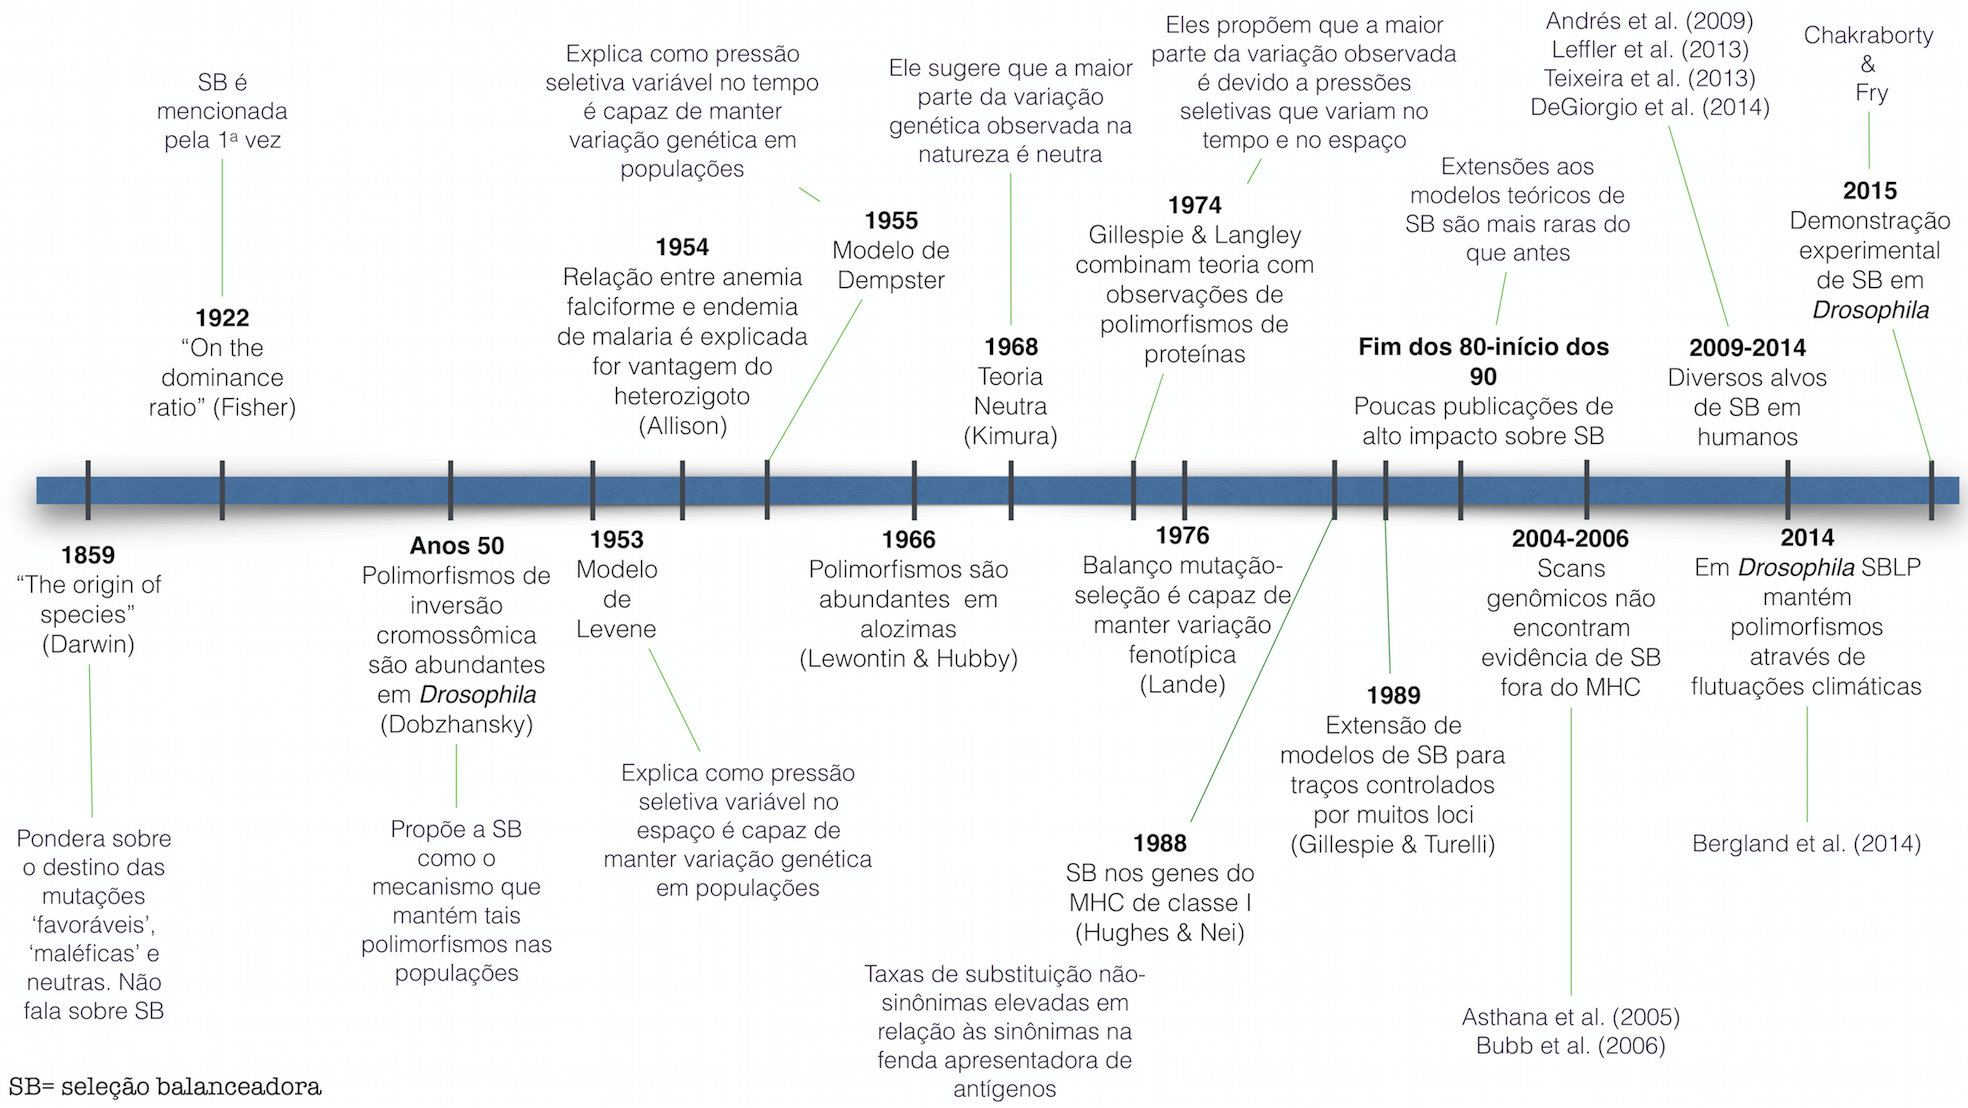
\includegraphics{chap1_folder/Figures/Figura_linha_do_tempo_v2.png}
\caption{\textbf{Linha do tempo do estudo da seleção balancedora} Adaptada a partir de \textcite{Gloss2016} resumindo as principais contribuições teóricas e empíricas para a compreensão da importância da seleção balanceadora para a manutenção de variação genética. SBLP, seleção balanceadora de longo prazo (ver texto).} %melhorar legenda pra essa fig.
\label{fig:LinhadoTempo}
\end{sidewaysfigure} 
%%%%%%%%%%%%%%%%%%%%%%%%%%%%%%%%%%%%%%%%%%%%%%%%%%%%%%%%%%%%%%%%%%%%%%%%%%%%%%%%%%%%%%%%%%%%%%%%%%%%%%%%%%%%%%%%%%
%%%%%%%%%%%%%%%%%%%%%%%%%%%%%%%%%%%%%%FIGURE FIGURE FIGURE%%%%%%%%%%%%%%%%%%%%%%%%%%%%%%%%%%%%%%%%%%%%%%%%%%%%%%%%
%%%%%%%%%%%%%%%%%%%%%%%%%%%%%%%%%%%%%%%%%%%%%%%%%%%%%%%%%%%%%%%%%%%%%%%%%%%%%%%%%%%%%%%%%%%%%%%%%%%%%%%%%%%%%%%%%%
%

    O "vigor do híbrido", ou heterose, é observado há séculos. Mendel percebeu que as ervilhas híbridas de seus estudos tinham altura média maior do que as das linhagens parentais \parencite{Crow1987a} e Darwin escreveu um livro inteiro sobre vigor do híbrido em plantas \parencite{Darwin1876}\footnote{Nesse livro, Darwin faz experimentos de auto-polinização e polinização cruzada em mais de 60 espécies de plantas e conclui que (na maior parte dos casos) a performance da prole resultante de auto-polinização é, para diversos traços, inferior.}. Apesar de ter sido observado frequentemente por criadores de plantas e animais, esse fenômeno só pôde ser corretamente interpretado após a re-descoberta das Leis de Mendel no início do século 20 (revisado em \cite{Crow1987a}), quando estabeleceu-se de forma definitiva que a variação genética é um dos fatores determinantes da variação fenotípica.
%

	Em 1922, Fisher \nocite{Fisher1922}menciona que, embora o vigor do híbrido fosse um fato, não era clara a razão biológica pela qual um heterozigoto qualquer seria mais apto que seu homozigoto correspondente. Fisher foi o primeiro a demonstrar como um equilíbrio de frequências entre dois alelos pode ser mantido em um loco sob vantagem de heterozigoto (ver página ~\pageref{sub:PressaoSeletivaConstante}). Ele propôs, ainda, que tal fenômeno deveria ser comum na natureza, e capaz de explicar tanto o vigor do híbrido quanto os efeitos deletérios às vezes observados em animais domesticados submetidos a endogamia. 
%

	Na medida em que começaram a surgir, desde a primeira metade do século 20, métodos capazes de acessar a variação genética diretamente -- uma propriedade que, começava-se então a perceber, era aparentemente ubíqua em populações naturais --, começou também a surgir um interesse crescente em se explicar os padrões de variação genética (revisado em \cite{Bamshad2003,Gloss2016}). Mesmo com métodos que para o geneticista de populações contemporâneo parecem bastante limitados (pois sempre forneciam subestimativas dos níveis reais de variabilidade genética das populações), variações genéticas já eram observadas desde meados do século 20, e sua persistência foi atribuída à ação da seleção balanceadora (\cite{Dobzhansky1937}). 

%[De novo, eu acho mais apropriado citar as fontes originais para essa
%frase, ou então "revisado em Gloss...". Os papers com esse argumento
%incluem o livro do Dobzhansky]

    O termo \enquote{seleção balanceadora} agregava todo e qualquer processo evolutivo que, de forma adaptativa, mantinha variação genética nas populações. Por exemplo, \textcite{Dobzhansky1937} observou polimorfismos na orientação de longos trechos de DNA em cromossomos de \emph{Drosophila} -- as chamadas \enquote{inversões cromossômicas} usando técnicas de coloração de cromossomos, muito antes de o sequenciamento de DNA ser possível -- e atribuiu à seleção balanceadora a manutenção de tais polimorfismos na natureza (Figura  ~\ref{fig:LinhadoTempo}).
%
%esse trecho tá copia quase literal. Preciso refrasear.

	Nessa época, no início do século 20, o interesse pela seleção balanceadora tinha múltiplas origens. Criadores de animais e plantas queriam maximizar a produtividade/performance, e o vigor do híbrido era observado, porém não totalmente compreendido. Dobzhansky, assim como Muller, estava preocupado com o potencial da espécie para continuar evoluindo. Entretanto, Muller tinha outra preocupação mais \enquote{urgente}: o impacto do aumento da taxa de mutação causada por radiação nas gerações futuras (revisado em \cite{Crow1987a}). Essas três preocupações giravam em torno do quanto a variabilidade genética na população depende da sobredominância\footnote{Esse termo, usado frequentemente como sinônimo para vantagem do heterozigoto, foi empregado originalmente para explicar a heterose em plantas \parencite{Hedrick2012}.}, i.e. em \emph{loci} nos quais o fenótipo do heterozigoto está além dos limites dos fenótipos dos dois homozigotos correspondentes\footnote{Essa é uma definição mais antiga de vantagem do heterozigoto \parencite{Crow1987a}. Outras serão mencionadas ao longo do texto.}.
%


Nos anos 60, \textcite{Lewontin1966} revelaram à comunidade científica que os níveis de variação genética em alozimas de \emph{Drosophila} eram muito mais altos do que o que se estimava ser a variabilidade genética nas populações até então analisadas (Figura ~\ref{fig:LinhadoTempo}). Suas descobertas foram baseadas em um novo método de detecção de polimorfismos -- a eletroforese de proteínas --, que permitia quantificar ainda mais variações do que as técnicas de coloração de cromossomos utilizadas por Dobzhansky uma década antes. A seleção balanceadora -- e, particularmente, a seleção que varia ao longo do tempo -- se consagrou então como uma explicação bastante popular para a manutenção de polimorfismos na natureza (revisado em \cite{Bamshad2003,Gloss2016}).
%

	É importante mencionar que o mecanismo principal de seleção balanceadora invocado para explicar os níveis de variação em \emph{Drosophila} era a heterogeneidade espacial nas pressões seletivas (\cite{Levene1953}), decorrente do fato de tais espécies ocuparem hábitats diversos: uma determinada variante não seria a mais adaptativa em todos os hábitats, assim levando à manutenção de polimorfismos na população (Figura ~\ref{fig:LinhadoTempo}). Mais tarde, \textcite{Dempster1955} mostrou que pressões seletivas que variam ao longo do tempo também podem manter variações genéticas (revisado em \cite{Gloss2016}). 
    
    Nas décadas seguintes, na medida em que modelos matemáticos foram sendo desenvolvidos no sentido de descrever tais regimes seletivos, evidências empíricas de sua ocorrência na natureza começaram a surgir (i.e,  \cite{Allison1954}). Nesse período, acreditava-se amplamente em uma teoria neo-Darwinista bastante \enquote{selecionista}, i.e, focada em seleção natural como o principal mecanismo capaz de alterar frequências alélicas e fenotípicas: as variantes seriam em sua grande maioria deletérias, e uma proporção menor seria vantajosa (Figura ~\ref{fig:ProportionMutations}). 



%[Há um pouco de peso excessivo no texto de Gloss. Considere, quando
%apropriado, citar fontes primárias]
%BDB: acho que melhorou agora. Verificar.

%%%%%%%%%%%%%%%%%%%%%%%%%%%%%%%%%%%%%%%%%%%%%%%%%%%%%%%%%%%%%%%%%%%%%%%%%%%%%%%%%%%%%%%%%%%%%%%%%%%%%%%%%%%%%%%%%%
%%%%%%%%%%%%%%%%%%%%%%%%%%%%%%%%%%%%%FIGURE FIGURE FIGURE%%%%%%%%%%%%%%%%%%%%%%%%%%%%%%%%%%%%%%%%%%%%%%%%%%%%%%%%%
%%%%%%%%%%%%%%%%%%%%%%%%%%%%%%%%%%%%%%%%%%%%%%%%%%%%%%%%%%%%%%%%%%%%%%%%%%%%%%%%%%%%%%%%%%%%%%%%%%%%%%%%%%%%%%%%%%
\begin{figure}[h]
\centering
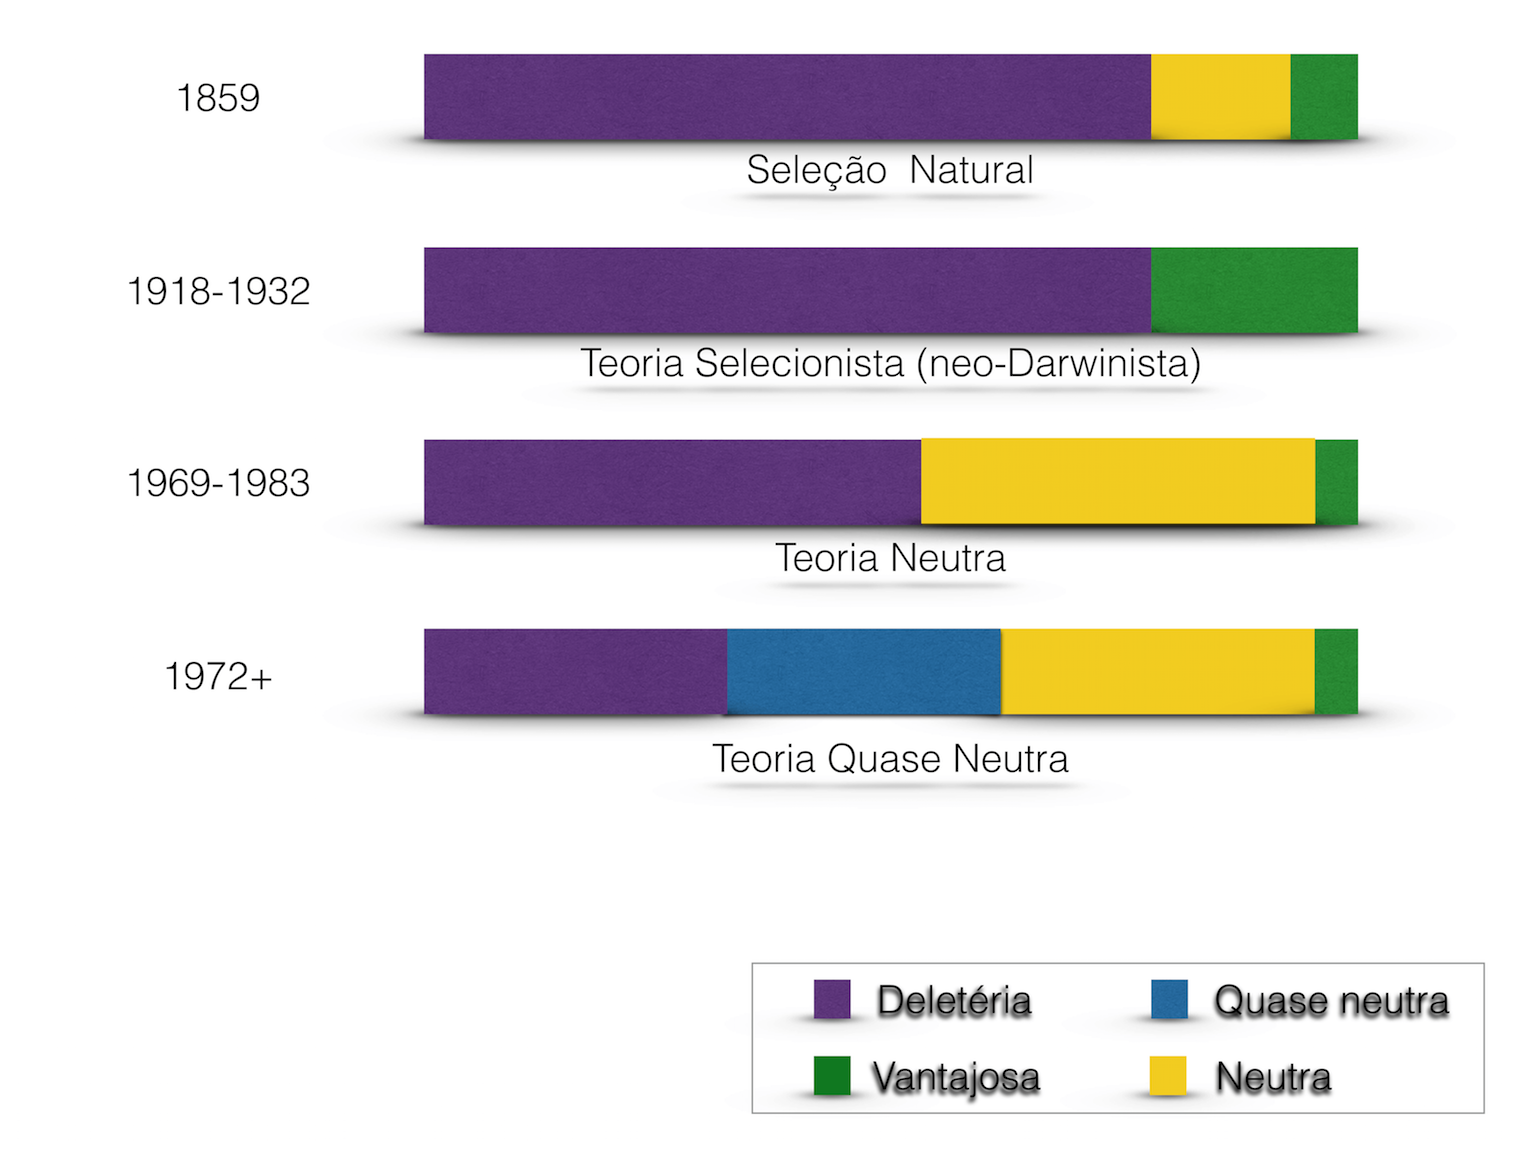
\includegraphics[height=7cm,keepaspectratio]{chap1_folder/Figures/proportion_mutations.png}
\caption{Modelos selecionista, neutro e quase neutro de evolução molecular. Figura adaptada a partir de \textcite{Bromham2003,Bernardi2007}. Em 1859, Darwin publica o livro "A origem das espécies", no qual descreve suas ideias sobre seleção natural\nocite{Darwin1979}. Darwin acredita que possam haver mutações neutras,  porém a maioria das mutações são deletérias e poucas são vantajosas. Na primeira metade do século 20 a seleção natural é conciliada com as bases do mecanismo molecular de herança (Neo-Darwinismo). Neste período, o foco selecionista aborda apenas mutações deletérias e vantajosas. Em 1968 Kimura publica a primeira versão do modelo neutro de evolução molecular (e uma atualização importante em 1983) e em 1973 Ohta \nocite{Ohta1973SlightlyEvolution} propõe o modelo quase neutro de evolução molecular. Esses dois últimos autores mostram que a deriva genética pode manter variantes neutras ou quase neutras nas populações. Ver também Figura ~\ref{fig:LinhadoTempo}.} 
\label{fig:ProportionMutations}
\end{figure}
%%%%%%%%%%%%%%%%%%%%%%%%%%%%%%%%%%%%%%%%%%%%%%%%%%%%%%%%%%%%%%%%%%%%%%%%%%%%%%%%%%%%%%%%%%%%%%%%%%%%%%%%%%%%%%%%%%
%%%%%%%%%%%%%%%%%%%%%%%%%%%%%%%%%%%%%FIGURE FIGURE FIGURE%%%%%%%%%%%%%%%%%%%%%%%%%%%%%%%%%%%%%%%%%%%%%%%%%%%%%%%%%
%%%%%%%%%%%%%%%%%%%%%%%%%%%%%%%%%%%%%%%%%%%%%%%%%%%%%%%%%%%%%%%%%%%%%%%%%%%%%%%%%%%%%%%%%%%%%%%%%%%%%%%%%%%%%%%%%%
%
%%%%%%%%%%%%%%%%%%%%%%%%%%%%%%%%%%%%%%%%%%%%%%%%%%%%%%%%%%%%%%%%%%%%%%%%%%%%%%%%%%%%%%%%%%%%%%%%%%%%%% %Problas com a parte acima: a referência Gloss & Whiteman é citada demais...preciso refrasear mais e incluir outras referências mais originais, em vez apenas o artigo de review. 

%%%%%%%%%%%%%%%%%%%%%%%%%%%%%%%%%%%%%%%%%%%%%%%%%%%%%%%%%%%%%%%%%%%%%%%%%%%%%%%%%%%%%%%%%%%%%%%%%%%%%%
\subsection{Teoria neutra da evolução molecular}%%%%%%%%%%%%%%%%%%%%%%%%%%%%%%%%%%%%%%%%%%%%%%%%%%%%%%
%%%%%%%%%%%%%%%%%%%%%%%%%%%%%%%%%%%%%%%%%%%%%%%%%%%%%%%%%%%%%%%%%%%%%%%%%%%%%%%%%%%%%%%%%%%%%%%%%%%%%%
%%%%%%%%%%%%%%%%%%%%%%%%%%%%%%%%%%%%%%%%%%%%%%%%%%%%%%%%%%%%%%%%%%%%%%%%%%%%%%%%%%%%%%%%%%%%%%%%%%%%%%
%tem muitos trechos repetitivos nesse parte sobre Teoria Neutra. Além disso, preciso mencionar o modelo quase neutro, mesmo que brevemente.

\label{sec:Kimura}
	Com a sensibilidade cada vez maior dos métodos moleculares em detectar os níveis de variabilidade (i.e, \cite{Lewontin1966}), constatou-se a abundância de polimorfismos\footnote{A presença de variantes fenotípicas discretas em uma população é chamada de polimorfismo. Os polimorfismos \enquote{visíveis} são, contudo, uma subestimativa da diversidade genética subjacente (\cite{Charlesworth2010}). Ao longo do texto, polimorfismos são diferentes alelos alelos existentes na população para um dado loco.} em populações naturais, o que levou a um grande desenvolvimento de modelos de seleção balanceadora \parencite{Gloss2016}. A Figura ~\ref{fig:LinhadoTempo} resume muitas dessas contribuições.
   
   Entretanto, esse entusiasmo foi contrabalanceado pela então recente \enquote{teoria neutra da evolução molecular}. Em seu livro divisor de águas para o campo da biologia evolutiva\footnote{\enquote{The Neutral Theory of Molecular Evolution (1983)} é a versão consultada aqui e amplamente usada em genética de populações, embora a teoria tenha sido proposta pela primeira vez antes \parencite{Kimura1968}.}, Kimura apresenta à comunidade científica a ideia que a principal causa das mudanças evolutivas no nível molecular -- i.e, mudanças no material genético \emph{per se} -- não é a seleção positiva darwiniana, mas a fixação aleatória de variantes neutras ou quase neutras (Figura ~\ref{fig:ProportionMutations}). 
  
% DM[Fica estranho se referir ao livro como "modelo nulo", que é o que o texto acima acaba implicando. No livro ele formaliza, revisa e argumenta a  favor do modelo, que acaba se tornando um modelo nulo.]
  %BB: EU nao estava dizendo que ele formaliza como modelo nulo. Isso tava na nota de rodapé, mas eu removi, dizendo apenas que é usado em genética de %populações. 
   
   
   Desde a primeira proposição da teoria neutra em 1968, Kimura enfrentou muitas críticas, em grande parte devido ao fato de a biologia evolutiva ter sido dominada por mais de meio século pela visão darwinista de que organismos se tornam progressivamente adaptados a seus ambientes pelo acúmulo de variantes benéficas (Figura ~\ref{fig:ProportionMutations}). Além disso, a teoria recebeu críticas de cunho técnico tais como a dificuldade de conciliar suas predições com alguns aspectos importantes dos dados gerados: variância elevada em taxas de evolução molecular, viés no uso de códons, evidência de seleção em estudo de genes específicos, entre outros. Essas críticas forçaram mudanças na teoria, que foi sendo revisada ao longo do tempo (\cite{Kimura1968,Kimura1983,Kimura1991}). Um outro desdobramento interessante foi a proposição da teoria \enquote{quase neutra} que, ao contrário da teoria neutra original, que tratava apenas de polimorfismos neutros e os muito deletérios, incorporou também os polimorfismos fracamente deletérios (\cite{Ohta1973SlightlyEvolution}) e os benéficos (\cite{Ohta1995,Ohta1996}; Figura ~\ref{fig:ProportionMutations}).
%

%[Mas as críticas mais "técnicas" e que acabaram forçando mudanças na teoria eram de aspectos mais precisos: dificuldade de conciliar as predições da teoria neutra com alguns aspectos importantes dos dados gerados: variância elevada em taxas de evolução molecular, viés no uso de códons, evidência de seleção em estudos de genes específicos, entre outros]


	Segundo a teoria neutra, variantes neutras, introduzidas por mutações, poderiam subir de frequência estocasticamente. Kimura (1968,1983)\nocite{Kimura1968,Kimura1983} apontou que, para contribuir para a adaptação, as mutações precisam ser mais do que benéficas: elas precisam escapar a perda por deriva, especialmente quando raras. Levando ambos os fatores em conta, Kimura concluiu que as mutações de efeito intermediário são as que mais provavelmente contribuem para a adaptação (revisado em \cite{Orr2005}). Adicionalmente, concluiu que a maior parte da variabilidade molecular intraespecífica, como por exemplo aquela manifestada pelos polimorfismos de proteínas, é essencialmente neutra, de forma que a maior parte dos alelos polimórficos são mantidos na espécie devido a um balanço entre mutação e extinção aleatória de alelos (\cite{Kimura1983}). 
%
%DM:[Depois me mostre onde ele explicita a predominância de mudanças associadas a "efeitos intermediários", não me lembrava disso]
%BDB: Diogo, na verdade eu li isso num review do ORR (2005): lá, ele diz que Kimura concluiu isso. Foi um erro não ter a referência aqui, vou adicionar. A referencia é : "The genetic theory of adaptation: a brief history" (4a página). Você acha que tá ok com a referência, ou discorda da ideia em si? Ou acha que complica demais esse trecho da Intro?


%
	
    Ao longo dos anos 60 e 70, por influência das ideias de Kimura, os geneticistas evolutivos ficaram cada vez mais convencidos de que muita -- se não a maior parte -- da evolução molecular reflete a fixação de mutações neutras ou quase neutras, e não benéficas. A teoria parecia ser capaz de explicar, através de processos estocásticos, a maior parte da variação observada dentro de populações. Nesse período, o estudo teórico dos mecanismos de evolução adaptativa -- seleção positiva e balanceadora -- diminuiu consideravelmente \parencite{Orr2005} (Figuras ~\ref{fig:LinhadoTempo} e ~\ref{fig:ProportionMutations}).
%
%DM:[A frase pode tb ser ampliada para incluir que a teoria neutra pareciaexplicar, através de processos estocásticos, a maior parte da variação observada dentro de populações]
%BDB: adicionei acima, veja se tá bom.

	Contudo, é interessante observar que a teoria neutra não se opõe à noção de que a evolução de forma e função possam ser guiadas por seleção darwiniana, mas destaca um outro aspecto do processo evolutivo ao enfatizar o papel crucial que as pressões mutacionais e a deriva genética possuem no nível molecular. \textcite{Kimura1983} define a teoria neutra como:
    
    \medskip

     \begin{quote} \enquote{\emph{(...)the theory that at the molecular level evolutionary changes and polymorphisms are mainly due to mutations that are nearly enough neutral with respect to natural selection that their behavior and fate are mainly determined by mutation and random drift.}} (Kimura 1983; primeiro capítulo). \end{quote}
%
\medskip

    A teoria olha os polimorfismos ao nível da proteína e do DNA como fases transitórias da evolução molecular e rejeita a noção de que a maior parte desses polimorfismos seja adaptativo e mantido na espécie devido a alguma forma de seleção balanceadora (Figura ~\ref{fig:ProportionMutations}). 	A teoria neutra prevê, portanto, que a maior parte das variantes genéticas são neutras; ela não rejeita, por outro lado, que as variantes genéticas \emph{funcionais} - aquelas que afetam os fenótipos, e que dentro de seu modelo, representam uma minoria da variação existente na natureza - poderiam ser mantidas por seleção balanceadora (\cite{Kimura1983,Gloss2016}).
%

	Com esse histórico -- não exaustivo -- sobre o tema da manutenção de diversidade nas populações, busquei apresentar os conceitos e distinção entre \emph{polimorfismos neutros}, mantidos com certa probabilidade simplesmente pela combinação dos efeitos de mutação, deriva, \enquote{efeito carona}\footnote{\emph{Genetic hitch-hiking}, processo através do qual mutações neutras -- ou, em alguns casos, deletérias -- mudam de frequência em uma população devido ao efeito de ligação genética com uma mutação selecionada (revisado em \cite{Cutter2013}). Esse tópico será abordado em maior detalhe na seção \enquote{Carga genética induzida por seleção balanceadora} e também no Capítulo 2.} e migração, e \emph{polimorfismos adaptativos}, que são mantidos por um ou mais mecanismos de seleção balanceadora\footnote{Embora a seleção positiva também atue sobre as mutações vantajosas ou adaptativas, ela tende a fixar tais variantes vantajosas na população, e portanto reduz, em vez de manter, a variabilidade genética.}. A seguir, detalharei cada um desses mecanismos. 
%
%
%OBSOLETE
%%%% "Adaptação não é seleção natural" (Orr 2005). %%%%%%%%%%%%%%%%%
%%%%%%%%%%%%%%%%%%%%%%%%%%%%%%%%%%%%%%%%%%%%%%%%%%%%%%%%%%%%%%%%%%%%
%%%%%%%%%%%%%%%%%%%%%%%%%%%%%%%%%%%%%%%%%%%%%%%%%%%%%%%%%%%%%%%%%%%%%%%%%%%%%%%%%%%%%%%%%%%%%%%%%%%%%%%%%%%%%%%%%%%%%%%%%%%%%%%%%%%%%%%%%%%%%%%%
%%%%%%%%%%%%%%%%%%%%%%%%%%%%%%%%%%%%%%%%%%%%%%%%%%%%%%%%%%%%%%%%%%%%%%%%%%%%%%%%%%%%%%%%%%%%%%%%%%%%%%%%%%%%%%%%%%%%%%%%%%%%%%%%%%%%%%%%%%%%%%%%%%%%%%%%%%%%%%%%%%%%%%%%%%%%%%%%%%%%%%%%%%%%%%%%%%%%%%%%%%%%%%%%%%%%%%%%%%%%%%%%%%%%%%%%%%%%%%%%%%%%%%%%%%%%%%%%%%%%%%%%%%%%%%%%%%%%%%%%%%%%%%%%
\subsection{Mecanismos de manutenção de diversidade adaptativa}%%%%%%%%%%%%%%%%%%%%%%%%%%%%%%%%%%%%%%%%%%%%%%%%%%%%%%%%%%%%%%%%%%%%%%%%%%%%%%%%%
%%%%%%%%%%%%%%%%%%%%%%%%%%%%%%%%%%%%%%%%%%%%%%%%%%%%%%%%%%%%%%%%%%%%%%%%%%%%%%%%%%%%%%%%%%%%%%%%%%%%%%%%%%%%%%%%%%%%%%%%%%%%%%%%%%%%%%%%%%%%%%%%
%%%%%%%%%%%%%%%%%%%%%%%%%%%%%%%%%%%%%%%%%%%%%%%%%%%%%%%%%%%%%%%%%%%%%%%%%%%%%%%%%%%%%%%%%%%%%%%%%%%%%%%%%%%%%%%%%%%%%%%%%%%%%%%%%%%%%%%%%%%%%%%%
%%%%%%%%%%%%%%%%%%%%%%%%%%%%%%%%%%%%%%%%%%%%%%%%%%%%%%%%%%%%%%%%%%%%%%%%%%%%%%%%%%%%%%%%%%%%%%%%%%%%%%%%%%%%%%%%%%%%%%%%%%%%%%%%%%%%%%%%%%%%%%%%

%\paragraph{Itens que devem constar nessa parte da introdução}
%\item prevalência de polimorfismos na natureza
%\item evolução neutra vs. adaptativa
%\item genética de populações etc
%\item carga genética, paradoxo etc
%\item Um pouco de nomenclatura, pra ficar bem claro o que quero dizer com seleção positiva, negativa (purificadora), balanceadora (diferente de diversificadora)
%\item mecanismos (dificuldade de destrinchar qual mecanismo está ocorrendo; nem sempre mutuamente excludentes)
%\item Manutenção de diversidade nas populações
%\item Mecanismo seletivo que aumenta diversidade
%\item Selection on standing variation
%\item Adaptive introgression? (avaliar se seria interessante incluir isso como tópico)
%\item assinaturas moleculares 
%\end{itemize}

%

	Dentro do pensamento evolutivo clássico não se previa um nível de variação que implicaria na existência de muitos casos de polimorfismos balanceados (Figura ~\ref{fig:LinhadoTempo}), i.e, aqueles mantidos em frequências intermediárias. Essa visão foi contestada pela descoberta de polimorfismos balanceados na natureza. Tal descoberta foi uma importante contribuição que ocorreu nos primórdios da genética de populações e que ajudou muito para uma melhor compreensão da evolução (\cite{Charlesworth2010}. 
%

	Níveis de variação genética, sabe-se hoje, são influenciados por fatores demográficos, tais como flutuações no tamanho populacional, estruturação, miscigenação e migração (\cite{Tishkoff2002})\footnote{Entretanto, por haver estocasticidade, em média a demografia afeta o genoma como um todo, e não apenas regiões específicas.}. Por outro lado, padrões de diversidade variam ao longo do genoma por diversos motivos, includindo taxas de mutação, taxas de recombinação, conversão gênica\footnote{Um tipo específico de recombinação, que resulta em uma troca não-recíproca de material genético, em que uma fita de DNA é usada para modificar a sequência de outra (\cite{Tishkoff2002}).} e processos seletivos (\cite{Tishkoff2002}). A classe de processos seletivos que levam a um aumento de diversidade genética vantajosa é conhecida como \enquote{seleção balanceadora} (\cite{Andres2011,Key2014b}). Refere-se a tais polimorfismos como \enquote{polimorfismos balanceados} \parencite{Charlesworth2010}.

	\emph{Seleção balanceadora} é um termo que engloba diversos mecanismos, os quais serão discutidos a seguir.

%%%%%%%%%%%%%%%%%%%%%%%%%%%%%%%%%%%%%%%%%%%%%%%%%%%%%%%%%%%%%%%%%%%%%%%%%%%%%%%%%%%%%%%%%%%%%%%%%%%%%%%%%%%%%%%%%%%%%%%%%%%%%%%%%%%%%%%%%%%%%%%%
%%%%%%%%%%%%%%%%%%%%%%%%%%%%%%%%%%%%%%%%%%%%%%%%%%%%%%%%%%%%%%%%%%%%%%%%%%%%%%%%%%%%%%%%%%%%%%%%%%%%%%%%%%%%%%%%%%%%%%%%%%%%%%%%%%%%%%%%%%%%%%%%
%%%%%%%%%%%%%%%%%%%%%%%%%%%%%%%%%%%%%%%%%%%%%%%%%%%%%%%%%%%%%%%%%%%%%%%%%%%%%%%%%%%%%%%%%%%%%%%%%%%%%%%%%%%%%%%%%%%%%%%%%%%%%%%%%%%%%%%%%%%%%%%%
\subsubsection{Aptidões constantes} %%%%%%%%%%%%%%%%%%%%%%%%%%%%%%%%%%%%%%%%%%%%%%%%%%%%%%%%%%%%%%%%%%%%%%%%%%%
%%%%%%%%%%%%%%%%%%%%%%%%%%%%%%%%%%%%%%%%%%%%%%%%%%%%%%%%%%%%%%%%%%%%%%%%%%%%%%%%%%%%%%%%%%%%%%%%%%%%%%%%%%%%%%%%%%%%%%%%%%%%%%%%%%%%%%%%%%%%%%%%
%%%%%%%%%%%%%%%%%%%%%%%%%%%%%%%%%%%%%%%%%%%%%%%%%%%%%%%%%%%%%%%%%%%%%%%%%%%%%%%%%%%%%%%%%%%%%%%%%%%%%%%%%%%%%%%%%%%%%%%%%%%%%%%%%%%%%%%%%%%%%%%%
%%%%%%%%%%%%%%%%%%%%%%%%%%%%%%%%%%%%%%%%%%%%%%%%%%%%%%%%%%%%%%%%%%%%%%%%%%%%%%%%%%%%%%%%%%%%%%%%%%%%%%%%%%%%%%%%%%%%%%%%%%%%%%%%%%%%%%%%%%%%%%%%
	 A modelagem de regimes de seleção balanceadora frequentemente é feita usando-se as aptidões dos genótipos sem que se especifique as causas subjacentes para as diferenças de fenótipo\footnote{Por exemplo, ver a seção de métodos do Capítulo 1.}. Embora seja uma estratégia útil, e na prática muitas das assinaturas genômicas deixadas pelos diferentes mecanismos de seleção balanceadora sejam as mesmas, é importante buscar entender quais aspectos biológicos de um organismo são capazes de determinar sua aptidão \parencite{Charlesworth2010}.

	\label{sub:PressaoSeletivaConstante}O modelo mais básico de seleção natural assume aptidões constantes dos genótipos (Figura ~\ref{fig:FrequenciaEquilibrio2}A). Para um sistema diploide e bi-alélico, as aptidões dos genótipos $A_{1}A_{1}$, $A_{1}A_{2}$ e $A_{2}A_{2}$ são dadas por $w_{11}$, $w_{12}$, e $w_{22}$, respectivamente. Em sistemas diploides, é comum utilizar o conceito de aptidões marginais dos alelos $A_{1}$ e $A_{2}$ para nos referirmos a uma média da aptidão de cada alelo considerando todos os genótipos em que ele aparece (i.e, homo e heterozigoto). 
    No cenário que estamos tratando aqui, embora $w_{11}$, $w_{12}$ e $w_{22}$ não mudem ao longo do tempo, as aptidões marginais continuam dependendo das frequências alélicas. Ou seja, é possível que as duas aptidões marginais se igualem, e que as frequências alélicas parem de mudar, atingindo um \emph{equilíbrio estável de frequências}. Chamamos a frequência de cada alelo, no equilíbrio, de \emph{frequência de equilíbrio}\footnote{No caso de locos bi-alélicos, a frequência de equilíbrio pode ser definida como a frequência do alelo menos frequente.}.  Interessantemente, os valores absolutos das aptidões dos genótipos são irrelevantes: apenas os valores relativos dos genótipos entram nas equações de seleção. Pode-se, portanto, definir um genótipo (e.g. o heterozigoto) como sendo o "padrão", e expressar as aptidões dos outros genótipos em relação a este, como apresentado a seguir \parencite{Charlesworth2010}.

%%%%%%%%%%%%%%%%%%%%%%%%%%%%%%%%%%%%%%%%%%%%%%%%%%%%%%%%%%%%%%%%%%%%%%%%%%%%%%%%%%%%%%%%%%%%%%%%%%%%%%%%%%%%%%%%%%%%%%%%%%%%%%%%%%%%%%%%%%%%%%%%
%%%%%%%%%%%%%%%%%%%%%%%%%%%%%%%%%%%%%%%%%%%%%%%%%%%%%%%%%%%%%%%%%%%%%%%%%%%%%%%%%%%%%%%%%%%%%%%%%%%%%%%%%%%%%%%%%%%%%%%%%%%%%%%%%%%%%%%%%%%%%%%%
%%%%%%FIGURE%%%%%FIGURE%%FIGURE%%%%%%%%%FIGURE%%%%%FIGURE%%FIGURE%%%%%%%%%FIGURE%%%%%FIGURE%%FIGURE%%%%%%%%%FIGURE%%%%%FIGURE%%FIGURE%%%FIGURE%%
%%%%%%%%%%%%%%%%%%%%%%%%%%%%%%%%%%%%%%%%%%%%%%%%%%%%%%%%%%%%%%%%%%%%%%%%%%%%%%%%%%%%%%%%%%%%%%%%%%%%%%%%%%%%%%%%%%%%%%%%%%%%%%%%%%%%%%%%%%%%%%%%
%%%%%%%%%%%%%%%%%%%%%%%%%%%%%%%%%%%%%%%%%%%%%%%%%%%%%%%%%%%%%%%%%%%%%%%%%%%%%%%%%%%%%%%%%%%%%%%%%%%%%%%%%%%%%%%%%%%%%%%%%%%%%%%%%%%%%%%%%%%%%%%%
\begin{figure}[h]
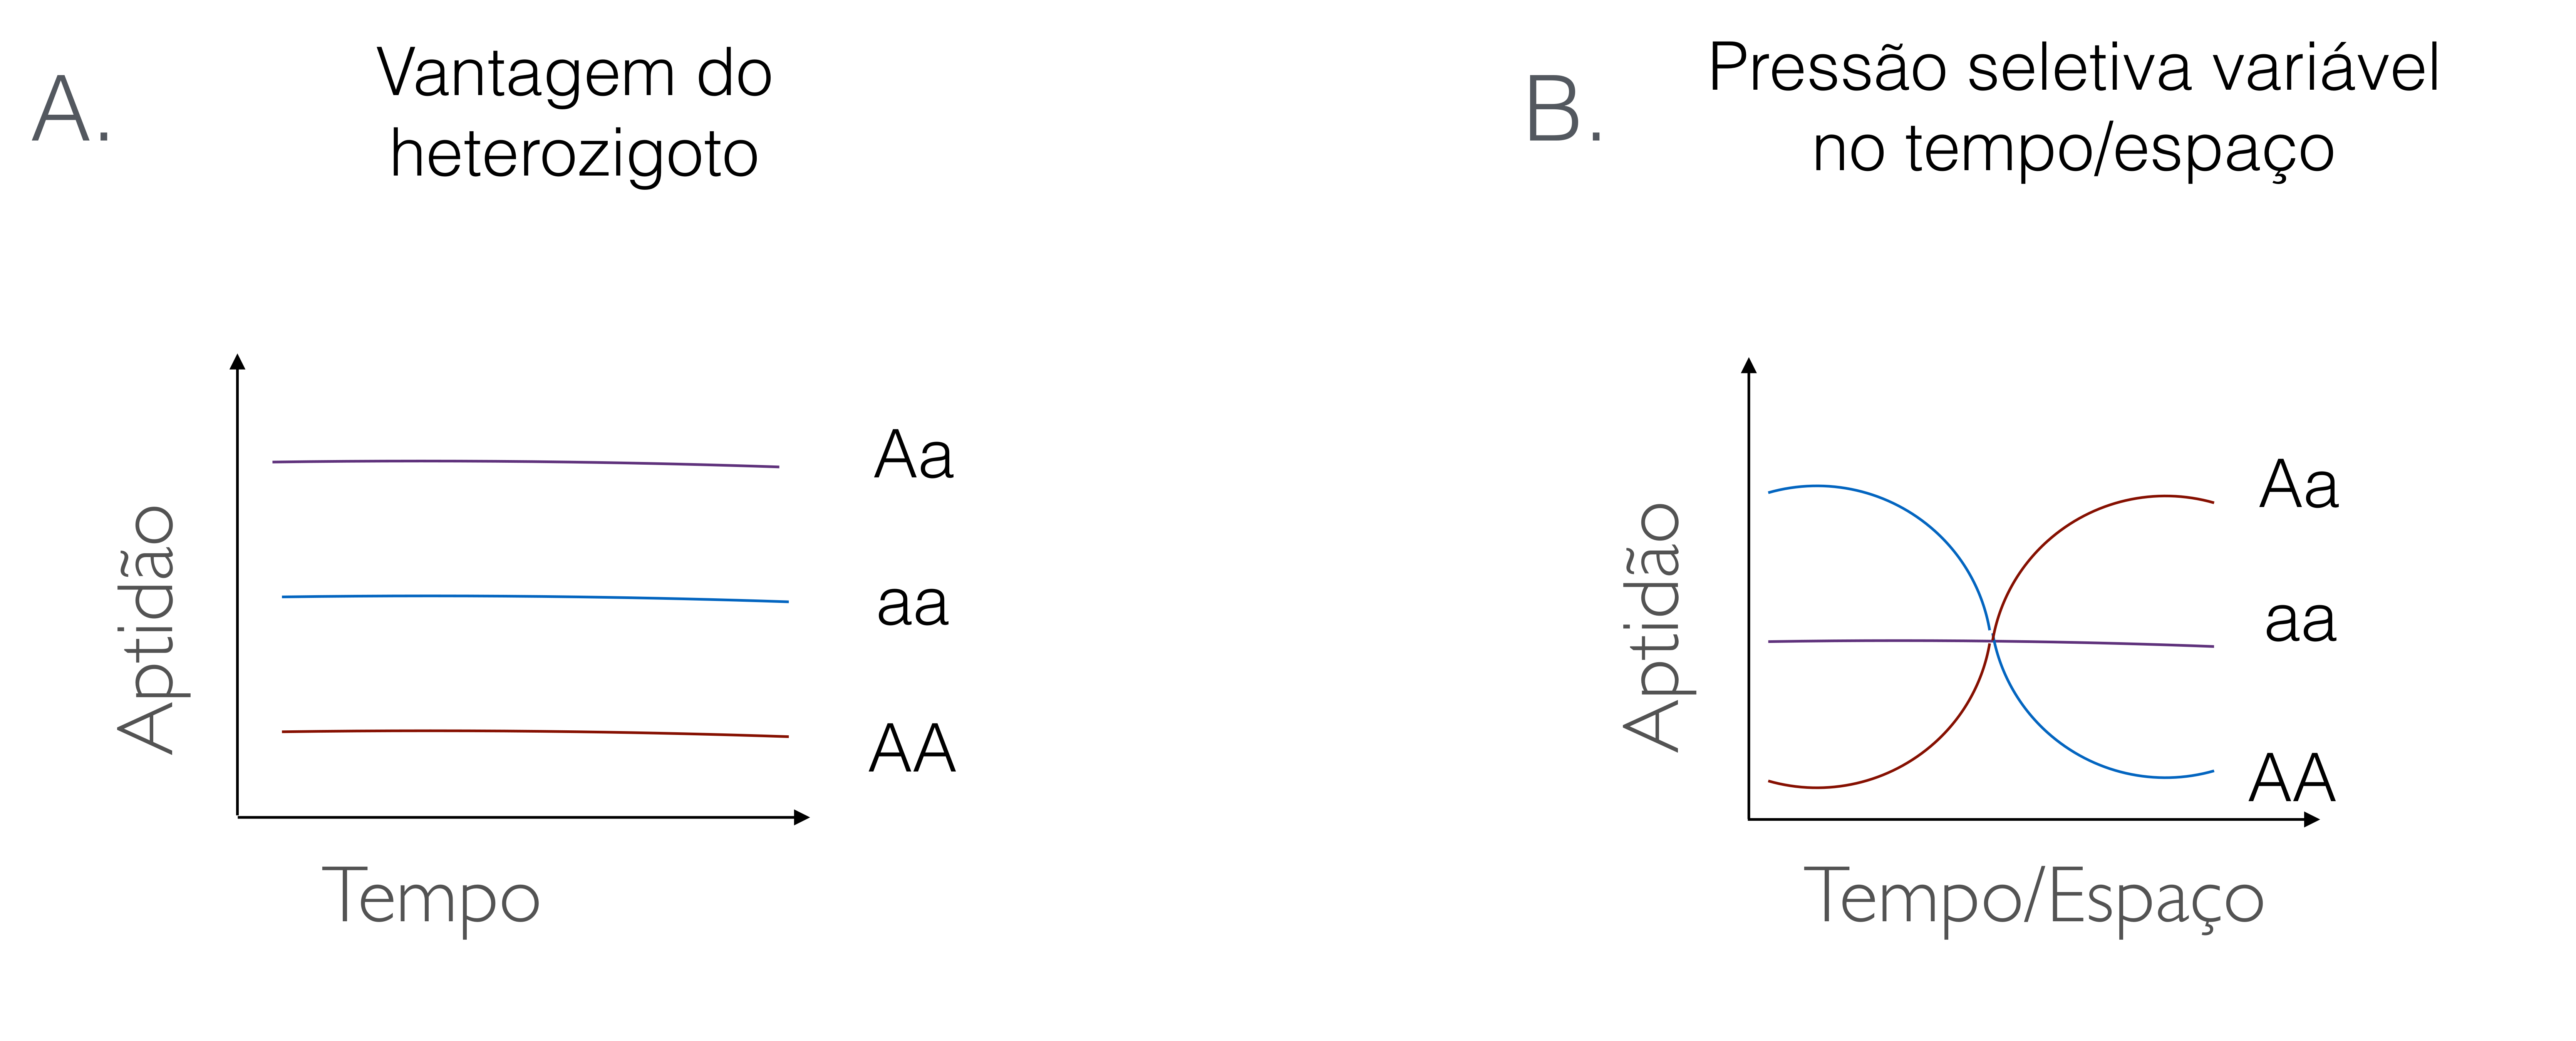
\includegraphics[height=6 cm,keepaspectratio]{chap1_folder/Figures/frequencia_equilibrio_2.png}
\caption{Uma possível estratégia para a identificação de instâncias de seleção balanceadora consiste em medir diferenças de aptidão entre classes genotípicas. Em (A), temos um cenário de sobredominância ou vantagem do heterozigoto, onde as aptidões dos genótipos são constantes mas a do heterozigoto é sempre mais alta que a de ambos os homozigotos. Nesse exemplo, os homozigotos têm aptidões distintas (sobredominância assimétrica). Em (B), temos um cenário de aptidões variáveis ao longo do espaço (por exemplo, diferentes hábitats ocupados por uma espécie) ou no tempo (quando um genótipo homozigoto tem maior aptidão em um dado momento, e reduz em gerações subsequentes). Figura adaptada de \textcite{Key2014b}.}
\label{fig:FrequenciaEquilibrio2}
\end{figure}

%verificar se essa legenda tá adequada.

%%%%%%%%%%%%%%%%%%%%%%%%%%%%%%%%%%%%%%%%%%%%%%%%%%%%%%%%%%%%%%%%%%%%%%%%%%%%%%%%%%%%%%%%%%%%%%%%%%%%%%%%%%%%%%%%%%%%%%%%%%%%%%%%%%%%%%%%%%%%%%%%
%%%%%%%%%%%%%%%%%%%%%%%%%%%%%%%%%%%%%%%%%%%%%%%%%%%%%%%%%%%%%%%%%%%%%%%%%%%%%%%%%%%%%%%%%%%%%%%%%%%%%%%%%%%%%%%%%%%%%%%%%%%%%%%%%%%%%%%%%%%%%%%%
%%%%%%FIGURE%%%%%FIGURE%%FIGURE%%%%%%%%%FIGURE%%%%%FIGURE%%FIGURE%%%%%%%%%FIGURE%%%%%FIGURE%%FIGURE%%%%%%%%%FIGURE%%%%%FIGURE%%FIGURE%%%FIGURE%%
%%%%%%%%%%%%%%%%%%%%%%%%%%%%%%%%%%%%%%%%%%%%%%%%%%%%%%%%%%%%%%%%%%%%%%%%%%%%%%%%%%%%%%%%%%%%%%%%%%%%%%%%%%%%%%%%%%%%%%%%%%%%%%%%%%%%%%%%%%%%%%%%
%%%%%%%%%%%%%%%%%%%%%%%%%%%%%%%%%%%%%%%%%%%%%%%%%%%%%%%%%%%%%%%%%%%%%%%%%%%%%%%%%%%%%%%%%%%%%%%%%%%%%%%%%%%%%%%%%%%%%%%%%%%%%%%%%%%%%%%%%%%%%%%%

\paragraph{Vantagem do heterozigoto}
Seguindo o modelo anterior, e usando frequências relativas dos genótipos, um cenário de vantagem do heterozigoto contendo dois alelos $A_{1}$ e $A_{2}$ com frequências $p$ e $q$ pode ser modelado da seguinte forma\footnote{A primeira demonstração e discussão de como um polimorfismo pode ser mantido por seleção, de forma bastante semelhante à apresentada aqui, foi feita no trabalho entitulado "\emph{On the dominance ratio}", de Fisher (1922). Ver a Figura ~\ref{fig:LinhadoTempo}.}:\\

%%%%%%%%%%%%%%%%%%%%%%%%%%%%%%%%%%%%%%%%%%%%%%%%%%%%%%%%%%%%%%%%%%%%%%%%%%%%%%%%%%%%%%%%%%%%%%%%%%%%%%%%%%%%%%%%%
%%% Equation %%%%%% Equation %%%%%% Equation %%%%%% Equation %%%%%% Equation %%%%%% Equation %%%%%% Equation %%%%
%%%%%%%%%%%%%%%%%%%%%%%%%%%%%%%%%%%%%%%%%%%%%%%%%%%%%%%%%%%%%%%%%%%%%%%%%%%%%%%%%%%%%%%%%%%%%%%%%%%%%%%%%%%%%%%%%
\centerline{$A_{1}A_{1}$\space\space\space\space $A_{2}A_{2}$\space\space\space\space $A_{2}A_{2}$} 

\centerline{$1-t$\space\space\space\space $1$\space\space\space\space \space\space$1-s$}

, onde $t$ e $s$ são os coeficientes seletivos dos alelos $A_{1}$ e $A_{2}$, respectivamente. Quando as duas aptidões marginais, de $A_{1}$ e $A_{2}$, são iguais ($qt=ps$), tem-se um \emph{equilíbrio polimórfico}, e a \emph{frequência de equilíbrio} é dada por:\\
\medskip
\centerline{$p_{\mathrm{eq}} = \frac{t}{t+s}; q_{\mathrm{eq}}=1-p_{\mathrm{eq}}$}
\medskip
%%%%%%%%%%%%%%%%%%%%%%%%%%%%%%%%%%%%%%%%%%%%%%%%%%%%%%%%%%%%%%%%%%%%%%%%%%%%%%%%%%%%%%%%%%%%%%%%%%%%%%%%%%%%%%%%
%%% Equation %%%%%% Equation %%%%%% Equation %%%%%% Equation %%%%%% Equation %%%%%% Equation %%%%%% Equation %%%%
%%%%%%%%%%%%%%%%%%%%%%%%%%%%%%%%%%%%%%%%%%%%%%%%%%%%%%%%%%%%%%%%%%%%%%%%%%%%%%%%%%%%%%%%%%%%%%%%%%%%%%%%%%%%%%%%%
\par 

%DM[Já que você inclui p e q na sua derivação, eu acho melhor na definição de frequência de equilíbrio você ter algo como p_eq e q_eq, colocando as duas e usando p e q]
%BDB: done. Você tem razão,até prque é apenas uma definição. No capítulo 1 a gente usa feq, mas será definida novamente lá.

	Através de vantagem do heterozigoto (também comumente chamada de sobredominância), polimorfismos podem ser mantidos em uma população devido à maior aptidão do genótipo heterozigoto em relação aos dois genótipos homozigotos, o que leva a um balanço de frequências entre as duas variantes \parencite{Andres2011,Fijarczyk2015,Key2014b}. A frequência de equilíbrio será 0.5 quando $s=t$, um cenário improvável, conhecido como sobredominância simétrica (Figura ~\ref{fig:FrequenciaEquilibrio}A), e $\neq 0.5$ quando $s \neq t$ (Figura ~\ref{fig:FrequenciaEquilibrio}B). Desde que a condição $qt=ps$ seja atendida, a frequência de equilíbrio é atingida independentemente de sua frequência inicial (Figura ~\ref{fig:FrequenciaEquilibrio}), i.e., o equilíbrio é \emph{estável}. No Capítulo 1, propomos uma estatística sumária que utiliza muitas dessas propriedades para detectar assinaturas de seleção balanceadora em dados genômicos (ver, por exemplo, Figuras 1 e 6 no Capítulo 1). 
%

	Um desdobramento interessante do modelo acima é que, supondo-se que um alelo $A_{2}$, inicialmente raro, entra em uma população inicialmente fixada para $A_{1}$  (por migração ou por mutação), então a proporção de genótipos $A_{2}A_{2}$ produzida por reprodução aleatória ($q^{2}$) é muito baixa comparada com a de heterozigotos \footnote{Pois $p \approx 1 $ e $2pq \approx  2q$}. Como genótipos $A_{2}A_{2}$ são inicialmente muito raros, a única condição compatível com um aumento de frequência de $A_{2}$ é que $A_{1}A_{2}$ tenha aptidão mais alta que $A_{1}A_{1}$, \emph{mesmo que} indivíduos $A_{2}A_{2}$ tenham aptidão muito reduzida. Assim, $A_{2}$ só vai aumentar de frequência até um certo ponto, uma vez que $A_{2}A_{2}$ é deletério. 
    
Com aptidão constante dos genótipos (Figura ~\ref{fig:FrequenciaEquilibrio2}A), a seleção balanceadora atuando sobre um só loco sempre maximiza a aptidão média de uma população com reprodução aleatória, ainda que, no caso de vantagem do heterozigoto, homozigotos com aptidões mais baixas sejam gerados por segregação mendeliana a cada geração (\cite{Charlesworth2010}). 

%%%%%%%%%%%%%%%%%%%%%%%%%%%%%%%%%%%%%%%%%%%%%%%%%%%%%%%%%%%%%%%%%%%%%%%%%%%%%%%%%%%%%%%%%%%%%%%%%%%%%%%%%%%%%%%%%%%%%%%%%%%%%%%%%%%%%%%%%%%%%%%%
%%%%%%%%%%%%%%%%%%%%%%%%%%%%%%%%%%%%%%%%%%%%%%%%%%%%%%%%%%%%%%%%%%%%%%%%%%%%%%%%%%%%%%%%%%%%%%%%%%%%%%%%%%%%%%%%%%%%%%%%%%%%%%%%%%%%%%%%%%%%%%%%
%%%%%%FIGURE%%%%%FIGURE%%FIGURE%%%%%%%%%FIGURE%%%%%FIGURE%%FIGURE%%%%%%%%%FIGURE%%%%%FIGURE%%FIGURE%%%%%%%%%FIGURE%%%%%FIGURE%%FIGURE%%%FIGURE%%
%%%%%%%%%%%%%%%%%%%%%%%%%%%%%%%%%%%%%%%%%%%%%%%%%%%%%%%%%%%%%%%%%%%%%%%%%%%%%%%%%%%%%%%%%%%%%%%%%%%%%%%%%%%%%%%%%%%%%%%%%%%%%%%%%%%%%%%%%%%%%%%%
%%%%%%%%%%%%%%%%%%%%%%%%%%%%%%%%%%%%%%%%%%%%%%%%%%%%%%%%%%%%%%%%%%%%%%%%%%%%%%%%%%%%%%%%%%%%%%%%%%%%%%%%%%%%%%%%%%%%%%%%%%%%%%%%%%%%%%%%%%%%%%%%

\begin{figure}[h]
\begin{center}
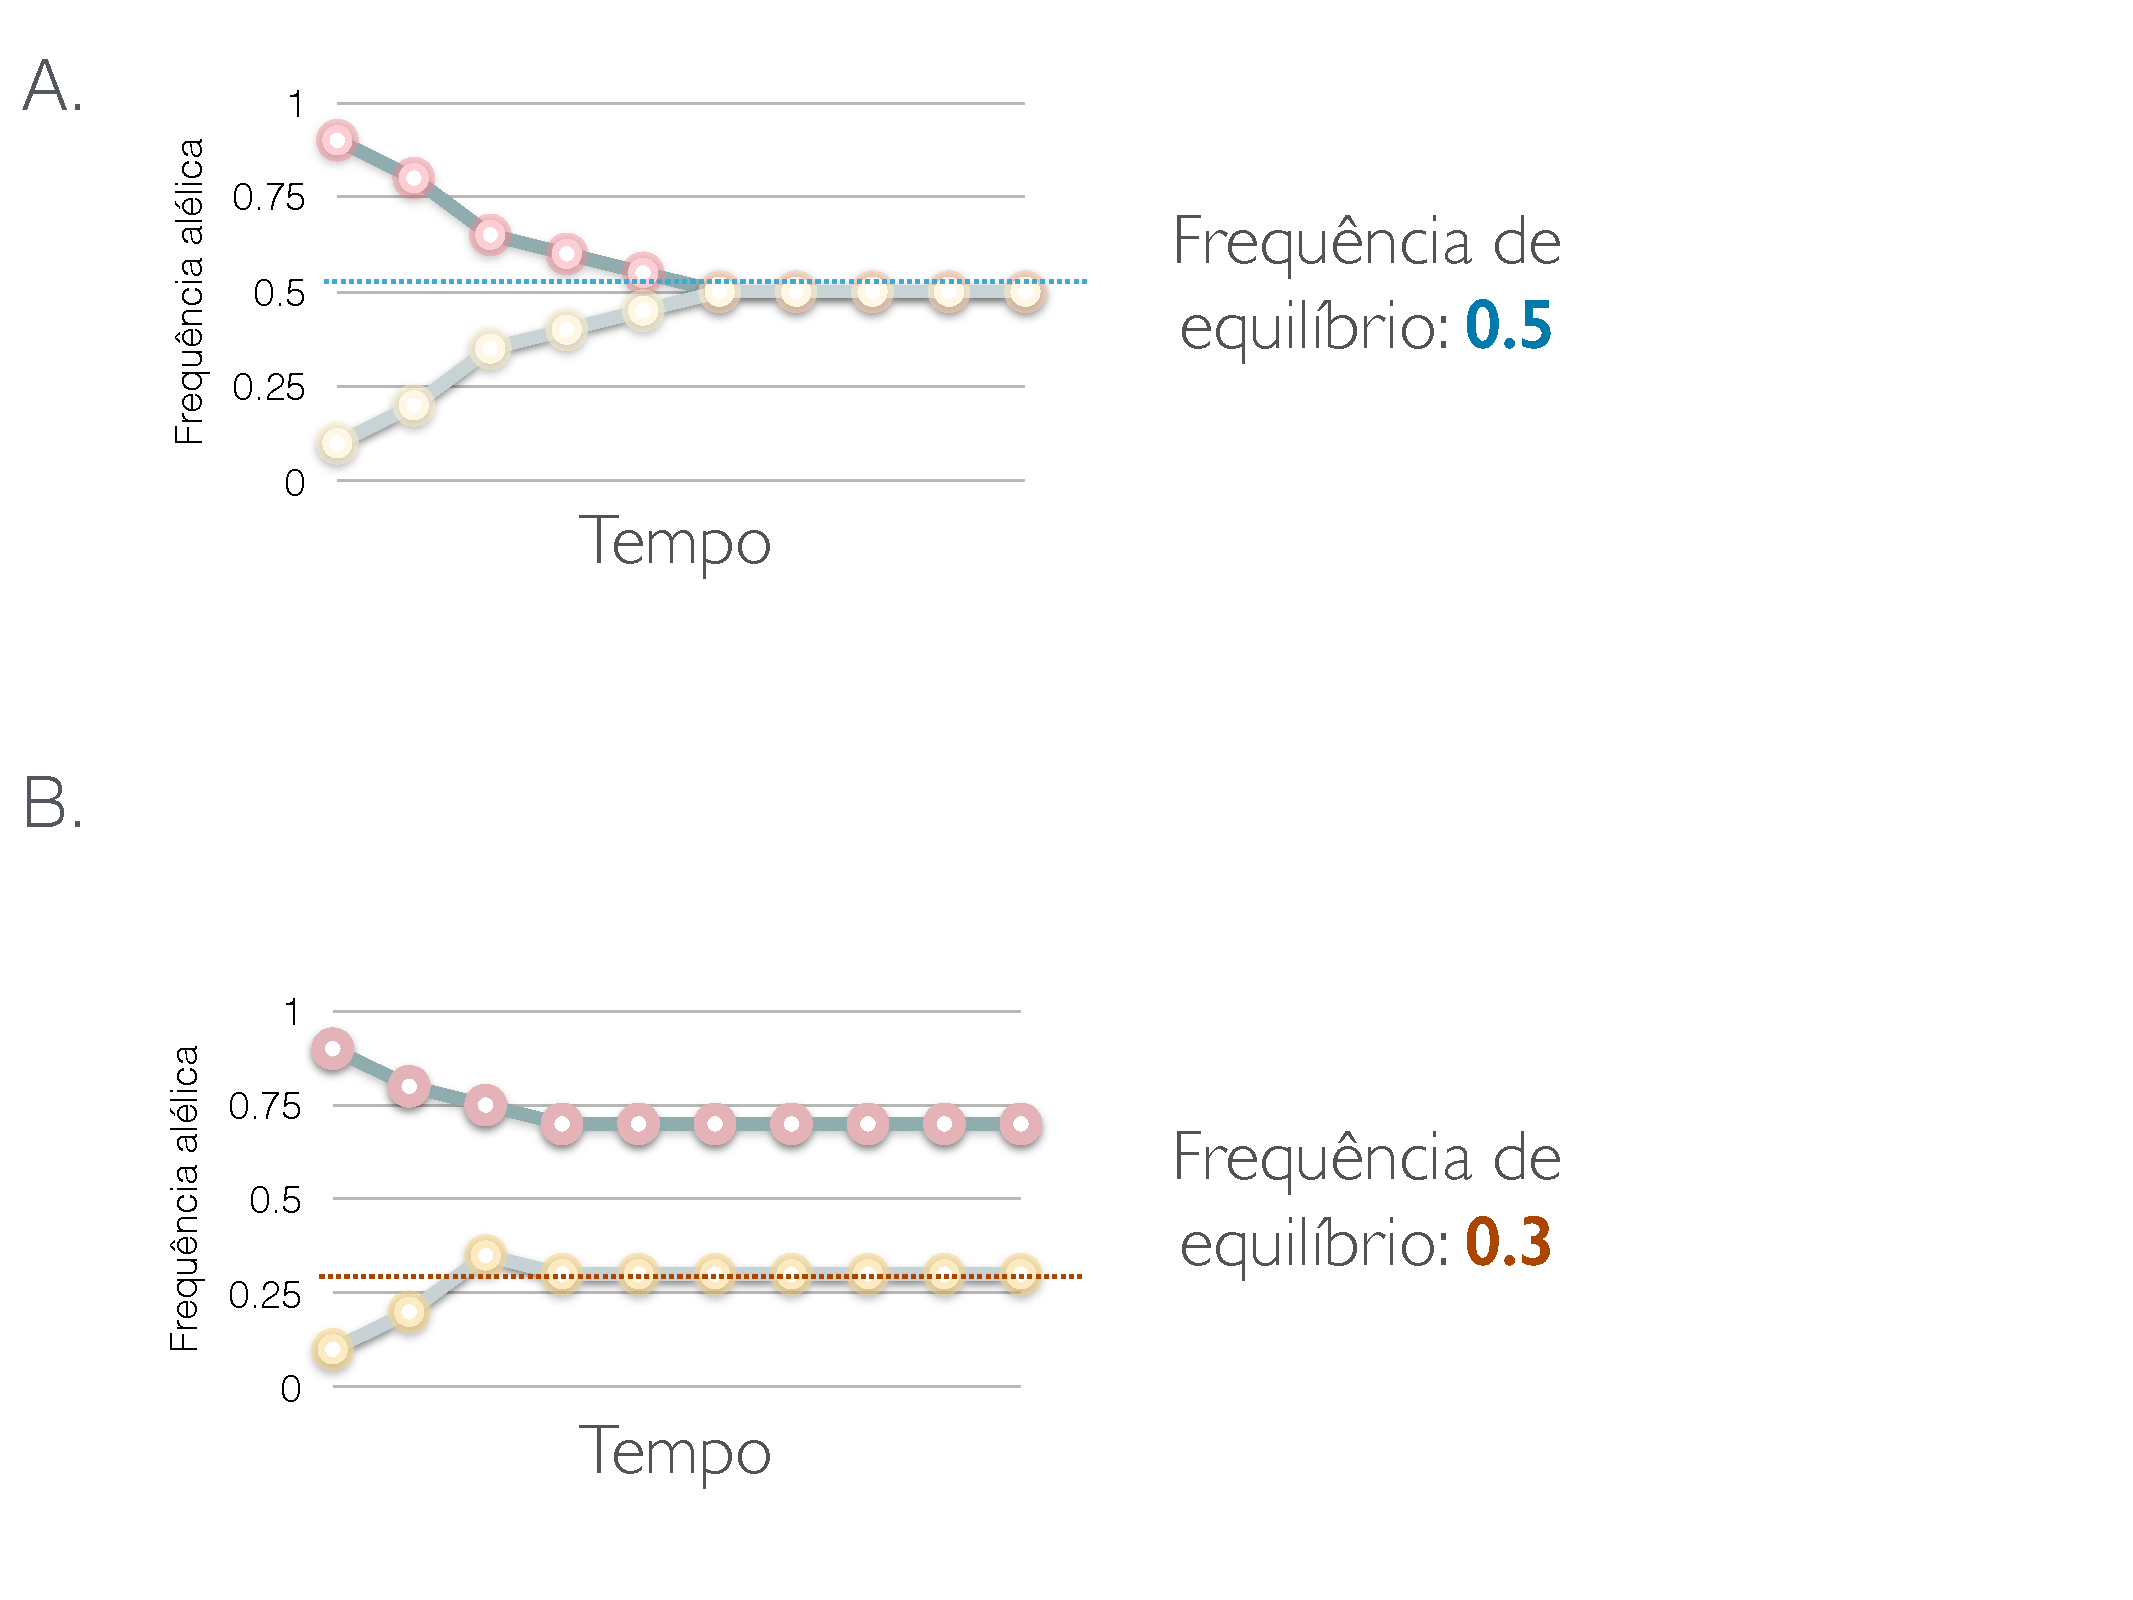
\includegraphics[width=12 cm,keepaspectratio]{chap1_folder/Figures/frequencia_equilibrio.pdf}
\caption{Independente da frequência inicial de cada alelo em um sistema bi-alélico com vantagem de heterozigoto, um equilíbrio pode ser atingido (desde que o alelo sobreviva a perda por deriva). Se as aptidões relativas dos dois genótipos homozigotos em relação ao heterozigoto são idênticas, o equilíbrio é atingido em uma frequência de 0.5 para cada alelo (\emph{A}). Se um dos genótipos homozigotos tem aptidão relativa maior do que o outro, a frequência de equilíbrio atingida será diferente 0.5 (\emph{B}, onde a frequência de equilíbrio é de 0.3 para um alelo e 0.7 para o outro, consequentemente). No Capítulo 1, um exemplo real de sobredominância assimétrica é apresentado (Página ~\pageref{page:HbS}).}
\label{fig:FrequenciaEquilibrio}
\end{center}
\end{figure}
%%%%%%%%%%%%%%%%%%%%%%%%%%%%%%%%%%%%%%%%%%%%%%%%%%%%%%%%%%%%%%%%%%%%%%%%%%%%%%%%%%%%%%%%%%%%%%%%%%%%%%%%%%%%%%%%%%%%%%%%%%%%%%%%%%%%%%%%%%%%%%%%
%%%%%%%%%%%%%%%%%%%%%%%%%%%%%%%%%%%%%%%%%%%%%%%%%%%%%%%%%%%%%%%%%%%%%%%%%%%%%%%%%%%%%%%%%%%%%%%%%%%%%%%%%%%%%%%%%%%%%%%%%%%%%%%%%%%%%%%%%%%%%%%%
%%%%%%FIGURE%%%%%FIGURE%%FIGURE%%%%%%%%%FIGURE%%%%%FIGURE%%FIGURE%%%%%%%%%FIGURE%%%%%FIGURE%%FIGURE%%%%%%%%%FIGURE%%%%%FIGURE%%FIGURE%%%FIGURE%%
%%%%%%%%%%%%%%%%%%%%%%%%%%%%%%%%%%%%%%%%%%%%%%%%%%%%%%%%%%%%%%%%%%%%%%%%%%%%%%%%%%%%%%%%%%%%%%%%%%%%%%%%%%%%%%%%%%%%%%%%%%%%%%%%%%%%%%%%%%%%%%%%
%%%%%%%%%%%%%%%%%%%%%%%%%%%%%%%%%%%%%%%%%%%%%%%%%%%%%%%%%%%%%%%%%%%%%%%%%%%%%%%%%%%%%%%%%%%%%%%%%%%%%%%%%%%%%%%%%%%%%%%%%%%%%%%%%%%%%%%%%%%%%%%%

%%%%%%%%%%%%%%%%%%%%%%%%%%%%%%%%%%%%%%%%%%%%%%%%%%%%%%%%%%%%%%%%%%%%%%%%%%%%%%%%%%%%%%%%%%%%%%%%%%%%%%%%%%%%%%%%%%%%%%%%%%%%%%%%%%%%%%%%%%%%%%%%
%%%%%%%%%%%%%%%%%%%%%%%%%%%%%%%%%%%%%%%%%%%%%%%%%%%%%%%%%%%%%%%%%%%%%%%%%%%%%%%%%%%%%%%%%%%%%%%%%%%%%%%%%%%%%%%%%%%%%%%%%%%%%%%%%%%%%%%%%%%%%%%%    
    
%
Devido a essa propriedade, \textcite{Sellis2011a} demonstraram, teoricamente, que é provável que esta seja a trajetória da maior parte das mutações adaptativas em diploides. Esse estado \enquote{balanceado} seria, por definição, muito frequente e de curta duração, e não deixaria assinaturas passíveis de serem captadas pelos métodos focados em assinaturas de seleção balanceadora de longa duração. Por outro lado, teria a vantagem de manter diversidade adaptativa nas populações -- mesmo que a curto prazo -- o que compensaria a perda de aptidão causada pelos homozigotos. Esse fenômeno poderia ser responsável por manter diversidade adaptativa nas populações, que por sua vez poderia ser usada prontamente pela seleção natural em casos de mudança repentina de pressão seletiva\footnote{Esse fenômeno, que vem sendo cada vez mais estudado, é chamado de \emph{selection on standing variation}.}. Embora seja uma proposição muito interessante, faltam evidências de empíricas para apoiá-la ou rejeitá-la.

%%%%%%%%%%%%%%%%%%%%%%%%%%%%%%%%%%%%%%%%%%%%%%%%%
%%%%%%%%%%%%%%%%%%%%%%%%%%%%%%%%%%%%%%%%%%%%%%%%%
\paragraph{Aptidão média} %%%%%%%%%%%%%%%%%%%%%%%
%%%%%%%%%%%%%%%%%%%%%%%%%%%%%%%%%%%%%%%%%%%%%%%%%
%%%%%%%%%%%%%%%%%%%%%%%%%%%%%%%%%%%%%%%%%%%%%%%%%
%
Seria lógico pensar que, em um cenário de vantagem do heterozigoto, a inevitável geração de homozigotos a cada geração por segregação mendeliana levaria a uma redução da aptidão média da população. Entretanto, esse não é o caso: a aptidão \emph{média} de uma população (i.e, considerando todos os genótipos e suas frequências) com reprodução aleatória e vantagem do heterozigoto \emph{atinge o seu máximo no equilíbrio}. Por isso, diz-se que a frequência de equilíbrio em um cenário de vantagem do heterozigoto é \emph{aquela que maximiza a aptidão média da população} (\cite{Charlesworth2010,Andres2011}). Portanto, embora a presença de homozigotos com baixa aptidão no caso da anemia falciforme, por exemplo, seja muito prejudicial para o indivíduo, a aptidão da população como um todo é mais alta quando indivíduos resistentes à malária são mantidos na população \parencite{Charlesworth2010, Wright1937}.
%
%%%%%%%%%%%%%%%%%%%%%%%%%%%%%%%%%%%%%%%%%%%%%%%%%%%%%%%%%%%%%%%%%%%%%%%%%%%%%%%%
%%%%%%%%%%%%%%%%%%%%%%%%%%%%%%%%%%%%%%%%%%%%%%%%%%%%%%%%%%%%%%%%%%%%%%%%%%%%%%%%
\paragraph{Seleção antagonista} %%%%%%%%%%%%%%%%%%%%%%%%%%%%%%%%%%%%%%%%%%%%%%%%
%%%%%%%%%%%%%%%%%%%%%%%%%%%%%%%%%%%%%%%%%%%%%%%%%%%%%%%%%%%%%%%%%%%%%%%%%%%%%%%%
%%%%%%%%%%%%%%%%%%%%%%%%%%%%%%%%%%%%%%%%%%%%%%%%%%%%%%%%%%%%%%%%%%%%%%%%%%%%%%%%

%ta confuso, a charleswrth so fala em pleiotropia antagonista, que essencialmente é equivalente a vantagem do heterozigoto, como eu tento colocar aqui, mas o artigo Connalon & Clark fala de seleção antagonista, colocando nao so pleiotropia, mas seleção variável no tempo e no espaço como exemplos...mas da forma como estou escrevendo, eu queria falar de fitness constantes e nao constantes... rever isso depois.


	Pressões seletivas \emph{opostas} entre diferentes contextos -- ambientes, sexo do indivíduo, componentes de aptidão e estágios de desenvolvimento -- podem gerar seleção antagonista ao nível genético-populacional \parencite{Connallon2013,Prout2000}. Alelos selecionados de forma antagonista são aqueles que aumentam a aptidão em um contexto, mas diminuem-na em outro. Quando os contextos são componentes individuais de aptidão, tem-se um cenário conhecido como "pleiotropia antagonista" \label{text:pleiotropia}, em que um mesmo loco afeta mais de um caráter, e para um deles um alelo é adaptativo, e para o outro, é deletério \parencite{Connallon2013}.
%

	Suponhamos dois componentes de aptidão: fertilidade e sobrevivência. Se os efeitos do homozigoto para uma dada mutação atuam em direções opostas nos dois caráteres, e o alelo favorável em relação a cada caráter é dominante sobre o alelo deletério, o resultado será um cenário essencialmente indistinguível daquele de vantagem de heterozigoto, em que o loco pode evoluir para ter frequências intermediárias através de seleção balanceadora. Tal cenário foi descrito pela primeira vez em um trabalho sobre evolução do envelhecimento (\cite{Williams1957}), em que se propôs que se um alelo causa alta fertilidade na juventude e envelhecimento precoce, o segundo efeito seria compensado pelo primeiro (revisado em \cite{Charlesworth2000}). 
 
	Entretanto, a caminhada até o equilíbrio seria lenta, requirindo dezenas de milhares de gerações, mesmo com coeficientes seletivos não muito baixos \parencite{Connallon2013}, o que implica que: (1) alelos próximos do equilíbrio devem ser relativamente antigos (ver discussão sobre escalas de tempo, abaixo); e (2) que as populações devem em geral estar longe do equilíbrio para loci sujeitos a esse regime \parencite{Connallon2013}.


\paragraph{Exemplos de vantagem do heterozigoto} 
Como na prática é muito difícil estabelecer inequivocamente qual (ou quais) mecanismo(s) de seleção balanceadora é responsável pela manutenção de um polimorfismo balanceado durante longas escalas de tempo, existem poucos exemplos não controversos de vantagem do heterozigoto nessa escala de tempo \parencite{Charlesworth2010}. 

%
	Os genes do MHC (HLA em humanos\footnote{\emph{Major histocompatibility complex} e \emph{Human leukocyte antigen}, respectivamente.}) são um possível exemplo de vantagem do heterozigoto. Heterozigotos para alelos de genes codificadores de moléculas apresentadoras de antígenos teriam a capacidade de responder a um repertório maior de antígenos, e, portanto, responder melhor a infecções \parencite{Doherty1975}. Existe, entretanto, uma vasta literatura que mostra as dificuldades de se diferenciar os mecanismos atuantes sobre os genes MHC e suas contribuições relativas\footnote{Ver Introdução e Discussão do artigo no Apêndice A.4 para uma discussão detalhada sobre este tópico.}. O cenário mais provável é que diversos mecanismos contribuíram, em diferentes pontos do espaço e do tempo, para a evolução desse sistema, e possivelmente concomitantemente. Por outro lado, é improvável que a vantagem do heterozigoto, apenas, seja capaz de explicar o número de alelos encontrados nos genes do MHC \parencite{DeBoer2004}.
   
%DM[Dada a forma como você desenvolve o parágrafo, os genes MHC não serevelam "um ótimo exemplo" no sentido de serem inequívocos, mas sim deserem um exemplo plausível e muito estudado. Mas o grau de controvérsiaque você apresenta sugere mudar a forma como o qualifica, substituindo "ótimo" por algo menos enfático e que capte mais o debate]
%BDB: verificar se tá melhor.
    
%
	Em escalas de tempo mais recentes (milhares de anos), o exemplo mais clássico é o da $\beta$ - hemoglobina defeituosa que acarreta em anemia falciforme ao portador da mutação, e sua relação com proteção à malária\footnote{Ver também Página ~\pageref{page:HbS}.}. Muitos outros exemplos de vantagem do heterozigoto são conhecidos com base em mensurações de aptidão de diferentes genótipos, por exemplo em animais domesticados -- tais como porcos, cachorros, cavalos, gatos e ovelhas. Em muitos casos, traços selecionados por seleção artificial e que resultam em fenótipos desejáveis, geram como consequência fenótipos indesejados nos homozigotos recessivos \parencite{Hedrick2012}. Um exemplo extremo é o da ausência de cauda no gato da raça Manx, que é o fenótipo heterozigoto (selecionado); em homozigose, a mutação é letal \parencite{Hedrick2012}. 

%DM:[Não fica claro o que é um estudo "de geração atual". Talvez omita essa frase e vá direot para "estudos com animais domesticados", ficará mais claro.]
%BDB: eu achei importante manter, pois não é so com animais domesticados. Tem estudos com daphnia, drosophila (como aquele que você me mandou, das enzimas que degradam alcool),etc. O que eu quero dzer é que são estudos de seleção balanceadora ocorrendo na geração presente, ou atual, mas eu não sabia como dizer isso em português. Veja se tá mais claro.
%
%%%%%%%%%%%%%%%%%%%%%%%%%%%%%%%%%%%%%%%%%%%%%%%%%%%%%%%%%%%%%%%%%%%%%%%%%%%%%%%%%%%%%%%%%%%%%%%%%%%%%%%%%%%
\subsubsection{Aptidões não constantes} %%%%%%%%%%%%%%%%%%%%%%%%%%%%%%%%%%%%%%%%%%%%%%%%%%%%%%%%%%%%%%%%%%%%%%%%%%%%%%%%%%%%%%%%%%%%%%%%%%%%%%%%%%%
%%%%%%%%%%%%%%%%%%%%%%%%%%%%%%%%%%%%%%%%%%%%%%%%%%%%%%%%%%%%%%%%%%%%%%%%%%%%%%%%%%%%%%%%%%%%%%%%%%%%%%%%%%%%%%%%%%%%%%%%%%%%%%%%%%%%%%%%%%%%%%%%
%%%%%%%%%%%%%%%%%%%%%%%%%%%%%%%%%%%%%%%%%%%%%%%%%%%%%%%%%%%%%%%%%%%%%%%%%%%%%%%%%%%%%%%%%%%%%%%%%%%%%%%%%%%%%%%%%%%%%%%%%%%%%%%%%%%%%%%%%%%%%%%%
%Vantagem do heterozigoto a pleiotropia antagonista
%apontar pra figura disso

Na prática, a premissa de aptidões que são constantes ao longo do tempo é pouco realista: a variabilidade genética pode ser mantida ativamente mesmo na ausência de qualquer forma de vantagem do heterozigoto (Figura ~\ref{fig:FrequenciaEquilibrio2}B).

\paragraph{Dependência de frequência negativa} 
%DM[Eu geralmente digo "Seleção dependente de frequência negativa", mas talvez seja um anglicismo meu]
%BDB: acei no ridley em português: ele diz simplesmente 'dependência negativa de frequência'. Eu achei melhor. o que você acha?
% Prefiro como acima, negativo é um qualificador de "dependente de frequência". Cuidado com o Ridley, há muita tradução errada por lá...

Assumimos novamente os genótipos $A_{1}A_{1}$, $A_{1}A_{2}$ e $A_{2}A_{2}$, e que $A_{1}$ é dominante, de forma que genótipos $A_{1}/-$ têm aptidão diferente de $A_{2}A_{2}$.  Se  $A_{1}/-$ tem aptidão maior do que $A_{2}A_{2}$ quando $A_{1}$ é raro, mas a aptidão diminui na medida em que $A1$ aumenta de frequência, tem-se um cenário de seleção com dependência de frequência (também chamada de vantagem do alelo raro). Ou seja, a aptidão marginal de um alelo é negativamente correlacionada à sua frequência na população, o que leva a um balanço estável das frequências de cada variante, onde nenhuma das duas é eliminada\footnote{Em geral, ao longo do texto, assume-se que um loco permite duas variantes, ou seja, é bi-alélico.} \parencite{Clarke1962,Charlesworth2010}. Aqui,  a manutenção do polimorfismo não requer vantagem do heterozigoto.

Como nesse caso as aptidões dependem das frequências dos genótipos, o argumento acima sobre a frequência de equilíbrio ser aquela que maximiza a aptidão média da população não procede neste caso: aqui, o equilíbrio estável não precisa, por definição, coincidir com o a aptidão média máxima \parencite{Charlesworth2010}.

% Acho que está tudo ok. Meu palpite é que o que confundiu Kelly e Débora é o "argumento acima", que fica ambíguo pois pode se referir ao item anterior ou ao parágrafo anterior, gerando confusão. Explicitando o modelo que você tem em mente a coisa ficará mais clara.

\paragraph{Exemplos de dependência de frequência}

É provável que cenários como aqueles descritos acima sejam bastante comuns em sistemas naturais. Um exemplo é a \emph{seleção apostática}, em que predadores exercem pressão seletiva sobre suas presas ao \enquote{aprenderem} enquanto caçam: esse cenário favorece presas com fenótipos raros (\cite{Clarke1962,Charlesworth2010}). Outro exemplo é o mimetismo batesiano, onde uma espécie modelo perigosa, ou impalatável, é mimetizada por outra espécie (não perigosa), que é sujeita a predação. Variantes raras da espécie mimética, que porventura se pareçam com a espécie modelo, se beneficiam por serem evitadas por predadores, e aumentam de frequência; esse aumento de frequência aumenta a chance de um predador comer a espécie mimética e associar seu padrão a um gosto agradável (\cite{Charlesworth2010}), assim diminuindo sua vantagem.

É importante salientar que esses exemplos não levam inevitavelmente a um polimorfismo balanceado: isso depende da relação entre aptidão e frequências dos genótipos. Mais ainda, ao contrário do que ocorre na vantagem do heterozigoto, o equilíbrio é instável: análises teóricas apontam que nesse tipo de regime seletivo a população oscilará permanentemente em torno da frequência de equilíbrio \parencite{Charlesworth2010}.

	Outro exemplo importante é o sistema de auto-incompatibilidade: plantas com capacidade de se auto-polinizar costumam ter os chamados locos \enquote{S}, que compõem, junto com os genes do MHC em vertebrados, um dos sistemas mais polimórficos em termos de número de alelos \parencite{Charlesworth2010}. Nos exemplos mais simples, uma planta com grãos de pólen \emph{S1} não pode fertilizar óvulos que também carregam alelos \emph{S1}; assim, todas as plantas são heterozigotas por definição, e um novo alelo que surge tem uma enorme vantagem seletiva, pois o pólen que o carrega poderá fertilizar qualquer planta da população. Nesse cenário, um equilíbrio poderia ser atingido se todos os heterozigotos tivessem a mesma frequência \parencite{Charlesworth2010}.
    
    Finalmente, outro exemplo é o da \enquote{corrida armamentista} entre hospedeiros e parasitas. No contexto de imunidade adquirida, um tipo comum de parasita provavelmente terá infectado uma grande proporção dos hospedeiros, que se tornam imunes a novas infecções. Assim, parasitas com novos tipos de antígenos têm uma vantagem dependente de frequência, acarretando altos níveis de polimorfismos na população de parasitas (\cite{Trachtenberg2003,Borghans2004,Slade1992,Spurgin2010}). 
    
    É provável que parte da diversidade observada nos genes MHC seja mantida desta forma, uma vez que diferentes variantes dos genes que codificam as moléculas apresentadoras de antígenos são capazes de apresentar um repertório determinado de epítopos, e novas variantes que surgem no hospedeiro podem ter uma vantagem dependente de frequência (\cite{Trachtenberg2003,Borghans2004}). Essa hipótese é corroborada pela diversidade particularmente alta na fenda apresentadora de antígeno das moléculas MHC \parencite{Hedrick2003} e por uma correlação entre diversidade de patógenos e variabilidade no MHC humano \parencite{Prugnolle2005}, mas, conforme mencionado anteriormente, o debate acerca dos mecanismos responsáveis pela diversidade dos genes MHC permanece acirrado.  

%%%%%%%%%%%%%%%%%%%%%%%%%%%%%%%%%%%%%%%%%%%%%%%%%%%%%%%%%%%%%%%%%%%%%%%%%%%%
%%%%%%%%%%%%%%%%%%%%%%%%%%%%%%%%%%%%%%%%%%%%%%%%%%%%%%%%%%%%%%%%%%%%%%%%%%%%
%%%%%%%%%%%%%%%%%%%%%%%%%%%%%%%%%%%%%%%%%%%%%%%%%%%%%%%%%%%%%%%%%%%%%%%%%%%%
\paragraph{Aptidões que variam no tempo}
%%%%%%%%%%%%%%%%%%%%%%%%%%%%%%%%%%%%%%%%%%%%%%%%%%%%%%%%%%%%%%%%%%%%%%%%%%%%
%%%%%%%%%%%%%%%%%%%%%%%%%%%%%%%%%%%%%%%%%%%%%%%%%%%%%%%%%%%%%%%%%%%%%%%%%%%%
%%%%%%%%%%%%%%%%%%%%%%%%%%%%%%%%%%%%%%%%%%%%%%%%%%%%%%%%%%%%%%%%%%%%%%%%%%%%

Podemos imaginar cenários em que um alelo tem má performance em uma geração, e boa na geração subsequente (Figura ~\ref{fig:FrequenciaEquilibrio2}B). Um bom exemplo aqui são as flutuações sazonais observadas por \textcite{Dobzhansky1937} em inversões cromossômicas de \emph{D. pseudoobscura} ao longo das estações do ano. Mais recentemente, \textcite{Bergland2014} detectaram centenas de loci (SNPs) em \emph{D. melanogaster} cujas frequências variam dramaticamente entre estações do ano\footnote{Cerca de 10 gerações por verão, e duas por inverno \parencite{Bergland2014}.}, e argumentam que tais polimorfismos estão sujeitos a forte pressão seletiva, variável ao longo do tempo, dado que eles estão associados a fenótipos que variam entre as estações e que tais polimorfismos respondem a variações climáticas. 

    De fato, a teoria prevê que \enquote{polimorfismos protegidos} (\cite{Charlesworth2010,Prout1968}) podem permanecer em uma população com aptidões que variam ao longo do tempo, desde que a média geométrica das aptidões do heterozigoto seja mais alta que a de ambos os homozigotos ao longo do espaço de tempo considerado \parencite{Bergland2014,Charlesworth2010,Gillespie1974}\footnote{Entretanto, no estudo de \textcite{Bergland2014} modelos mais realistas foram considerados, que levam em conta a possibilidade de gerações que se sobrepõem, múltiplos loci ligados e uma combinação de variações espaciais e temporais nas pressões seletivas (todos compatíveis com \emph{D. melanogaster}), uma discussão além dos objetivos desta introdução.}.

%%%%%%%%%%%%%%%%%%%%%%%%%%%%%%%%%%%%%%%%%%%%%%%%%%%%%%%%%%%%%%%%%%%%%%%%%%%%
%%%%%%%%%%%%%%%%%%%%%%%%%%%%%%%%%%%%%%%%%%%%%%%%%%%%%%%%%%%%%%%%%%%%%%%%%%%%
\paragraph{Aptidões que variam no espaço}
%%%%%%%%%%%%%%%%%%%%%%%%%%%%%%%%%%%%%%%%%%%%%%%%%%%%%%%%%%%%%%%%%%%%%%%%%%%%
%%%%%%%%%%%%%%%%%%%%%%%%%%%%%%%%%%%%%%%%%%%%%%%%%%%%%%%%%%%%%%%%%%%%%%%%%%%%
Um polimorfismo protegido também pode ser mantido em ambientes que variam ao longo do espaço (Figura ~\ref{fig:FrequenciaEquilibrio2}B), sob as condições previstas no modelo de \textcite{Levene1953} (ver Figura ~\ref{fig:LinhadoTempo}), se: (a) a aptidão relativa dos genótipos varia entre diferentes nichos ocupados pela espécie; (b) toda a seleção ocorre dentro de cada nicho, e (c) a reprodução ocorre aleatoriamente entre os indivíduos de cada nicho.

Com alguma abstração, podemos também incluir aqui casos em que existem aptidões diferentes para um dado genótipo considerando os dois sexos: se alelos $A_{1}$ e $A_{2}$ têm efeitos opostos sobre a aptidão de machos e fêmeas (antagonismo sexual), polimorfismos podem ser mantidos na ausência de vantagem do heterozigoto\footnote{Ver também Página ~\pageref{text:pleiotropia}, onde o cenário de pleiotropia antagonista foi definido junto com o de vantagem de heterozigoto, pois ambos os mecanismos resultam em assinaturas indistinguíveis.}. Em \emph{D. melanogaster}, estima-se que 8\% dos genes têm padrões compatíveis com esse tipo de seleção \parencite{Innocenti2010}.

%[Isso não encaixaria melhor no trecho que trata de antagonistic pleiotropoy?]
%não ao meu ver. Antagonistic pleiotropy é um caso de pressão seletiva que varia 'entre componentes', mas refere-se especificamente a componentes de fitness. Já antagonismo sexual é um caso de antagonismo, mas não de pleiotropia. Concorda? Eu escolhi aqui o jeito que Charlesworth & Charlesworth definem, mas no paper Connalong e Clark eles botam tudo isso como 'seleção antagonista'. O que vc acha? Pus uma nota de rodapé remetendo a esse outro momento do texto. Veja o que acha. 

No caso de pressões seletivas que variam ao longo do espaço ocupado por uma espécie, a existência ou não de uma frequência de equilíbrio depende não apenas da relação entre as aptidões dos diversos alelos entre os ambientes, mas da proporção de indivíduos alocados a cada ambiente e da quantidade de fluxo gênico entre os ambientes \parencite{Gloss2016,Charlesworth2010}. Sendo assim, nesse mecanismo a manutenção de polimorfismos a longo-prazo pode ou não ocorrer.

Em muitos dos casos documentados de seleção balanceadora de curto e longo prazo (i.e, que não são detectados com base em estudos de geração atual), é difícil ou impossível determinar qual dos mecanismos  acima definidos é responsável pelo padrão observado. Ou seja, a detecção de assinaturas genômicas compatíveis com regimes seletivos de seleção balanceadora não permite diferenciar qual mecanismo é responsável pelo padrão observado (ver discussão no próximo item). Além disso, múltiplos mecanismos podem ter atuado simultaneamente ou em diferentes momentos ao longo da história evolutiva \parencite{Hedrick2012}, como é o caso do MHC.


%%%%%%%%%%%%%%%%%%%%%%%%%%%%%%%%%%%%%%%%%%%%%%%%%%%%%%%%%%%%%%%%%%%%%%%%%%%%%%%%%%%%%%%%%%%%%%%%%%%%
%%%%%%%%%%%%%%%%%%%%%%%%%%%%%%%%%%%%%%%%%%%%% SEGUNDA PARTE DA INTRODUÇÃO %%%%%%%%%%%%%%%%%%%%%%%%%%%%%%%%%%%%%%%%
%%%%%%%%%%%%%%%%%%%%%%%%%%%%%%%%%%%%%%%%%%%%%%%%%%%%%%%%%%%%%%%%%%%%%%%%%%%%%%%%%%%%%%%%%%%%%%%%%%%%%%%%%%%%%%%%%%%%%%%%%%%%%%%%%%%%%%%%%%%%%%%%
%%%%%%%%%%%%%%%%%%%%%%%%%%%%%%%%%%%%%%%%%%%%%%%%%%%%%%%%%%%%%%%%%%%%%%%%%%%%%%%%%%%%%%%%%%%%%%%%%%%%%%%%%%%%%%%%%%%%%%%%%%%%%%%%%%%%%%%%%%%%%%%%
\section{Evolução adaptativa no genoma humano} %%%%%%%%%%%%%%%%%%%%%%%%%%%%%%%%%%%%%%%%%%%%%%%%%%%%%%%%%%%%%%%%%%%%%%%%%%%%%%%%%%%%%%%%%%%%%%%%%
%%%%%%%%%%%%%%%%%%%%%%%%%%%%%%%%%%%%%%%%%%%%%%%%%%%%%%%%%%%%%%%%%%%%%%%%%%%%%%%%%%%%%%%%%%%%%%%%%%%%%%%%%%%%%%%%%%%%%%%%%%%%%%%%%%%%%%%%%%%%%%%%
%%%%%%%%%%%%%%%%%%%%%%%%%%%%%%%%%%%%%%%%%%%%%%%%%%%%%%%%%%%%%%%%%%%%%%%%%%%%%%%%%%%%%%%%%%%%%%%%%%%%%%%%%%%%%%%%%%%%%%%%%%%%%%%%%%%%%%%%%%%%%%%%
%%%%%%%%%%%%%%%%%%%%%%%%%%%%%%%%%%%%%%%%%%%%%%%%%%%%%%%%%%%%%%%%%%%%%%%%%%%%%%%%%%%%%%%%%%%%%%%%%%%%%%%%%%%%%%%%%%%%%%%%%%%%%%%%%%%%%%%%%%%%%%%%
%gancho
%%%%%%%%%%%%%%%%%%%%%%%
%%%%%%%%%%%%%%%%%%%%%%%
\medskip
\begin{quotation}
\enquote{\emph{It is easy to invent a selectionist explanation for almost any specific observation; proving it is another story. Such facile explanatory excesses can be avoided by being more quantitative.}}   (\cite{Kimura1983})
\end{quotation}
\medskip
%%%%%%%%%%%%%%%%%%%%%%%
%%%%%%%%%%%%%%%%%%%%%%%
%esse seria um gancho pro tópico das assinaturas, e testes estatísticos destinados a rejeitar a hipótese numa (testes de neutralidade).
%reformular e focar mais em balanceadora do que em positiva.
%
	Durante décadas, o esforço de detectar casos de seleção positiva através do exame individual de genes candidatos resultou em alguns casos bem documentados, como o dos genes associados à persistência da enzima lactase em adultos (e.g. \cite{Bersaglieri2004}) e à pigmentação da pele em humanos (\cite{Jablonski2010}). Até recentemente, essa abordagem era a única forma prática de encontrar alvos de seleção positiva em humanos \parencite{Sabeti2006}. 

    Nos últimos 15 anos, abordagens genômicas tornaram-se populares, e houve uma explosão de \emph{scans} genômicos\footnote{Em um \emph{scan} genômico, uma estatística de interesse é calculada em janelas do genoma, e destaca-se aquelas que estão nos extremos empíricos da estatística e/ou além de algum limiar definido com base em simulações neutras.} em busca de assinaturas de seleção positiva no genoma humano (\cite{Bamshad2003,Bustamante2005,Enard2010,Fay2001,Nielsen2005,Sabeti2006,Sabeti2007}). Até 2009, 21 \emph{scans} para seleção positiva em humanos já haviam sido feitos (revisado em \cite{Akey2009}).
    
	Abordagens genômicas têm a vantagem de possibilitar a compreensão do impacto da seleção natural ao longo de todo o genoma e de inferir categorias funcionais mais sujeitas à ação da seleção positiva em humanos \parencite{Sabeti2006}. Graças à grande quantidade de \emph{scans} genômicos em busca de assinaturas de seleção positiva, sabe-se hoje que muitos dos genes com tais assinaturas estão relacionados com certas categorias: \enquote{imunidade e defesa}, \enquote{percepção sensorial} e \enquote{imunidade mediada por células T}, \enquote{gametogênese}, \enquote{espermatogênese e mobilidade} \parencite{Harris2006,Nielsen2005a}. Para as regiões não-codificadoras, destacam-se processos biológicos como \enquote{neurogênese}, \enquote{outras atividades neuronais} e \enquote{desenvolvimento muscular} \parencite{Haygood2010}.
%esse resultado parece muito suspeito...são genes grandes.

%Os testes de hipóteses explícitos de seleção positiva representam um amadurecimento dos estudos empíricos de seleção natural, que se desenvolveram notavelmente nas duas últimas décadas, tanto na abordagem morfológica quanto na genética (veja, por exemplo, Yang and Bielawski, 2000; Yang, 1998; Pickrell et al., 2009; Pritchard et al., 2010; Yang and Swanson, 2002). Uma vez que tornou-se claro que a seleção positiva foi comum na linhagem humana, para regiões codificadoras e não-codificadoras, questões relativas às consequências(em escala genômica) da seleção positiva começaram a ser investigadas.

%%%%%%%%%%%%%%%%%%%%%%%%%%%%%%%%%%%%%%%%%%%%%%%%%%%%%%%%%%%%%%%%%%%%%%%%%%%%%%%%%%%%%%%%%%%%%%%%%%%%%%%%%%%%%%%%%%%%%%%%%%%%%%%%%%%%%%%%%%%%%%%%
%%%%%%%%%%%%%%%%%%%%%%%%%%%%%%%%%%%%%%%%%%%%%%%%%%%%%%%%%%%%%%%%%%%%%%%%%%%%%%%%%%%%%%%%%%%%%%%%%%%%%%%%%%%%%%%%%%%%%%%%%%%%%%%%%%%%%%%%%%%%%%%%
\subsection{Assinaturas de seleção balanceadora} %%%%%%%%%%%%%%%%%%%%%%%%%%%%%%%%%%%%%%%%%%%%%%%%%%%%%%%%%%%%%%%%%%%%%%%%%%%%%%%%%%%%%%%%%%%%%%%
%%%%%%%%%%%%%%%%%%%%%%%%%%%%%%%%%%%%%%%%%%%%%%%%%%%%%%%%%%%%%%%%%%%%%%%%%%%%%%%%%%%%%%%%%%%%%%%%%%%%%%%%%%%%%%%%%%%%%%%%%%%%%%%%%%%%%%%%%%%%%%%%
%%%%%%%%%%%%%%%%%%%%%%%%%%%%%%%%%%%%%%%%%%%%%%%%%%%%%%%%%%%%%%%%%%%%%%%%%%%%%%%%%%%%%%%%%%%%%%%%%%%%%%%%%%%%%%%%%%%%%%%%%%%%%%%%%%%%%%%%%%%%%%%%

%tem muita coisa (demais) do Hedrick 2012. preciso misturar e dar um refraseada.

%isso aqui ta uma nagunça, pois fui transferindo trechos de outras seções pra cá. Preciso ler tudo e organizar.



	Desde a proposição da teoria neutra, muitos testes para seleção balanceadora no passado recente\footnote{Na literatura, frequentemente usa-se a expressão \enquote{seleção balanceadora de curto prazo} (últimos milhares de anos).} foram desenvolvidos. Por usarem o modelo neutro como modelo nulo, testes usados para detectar assinaturas de seleção natural são também chamados de "testes de neutralidade"\footnote{Ver página ~\pageref{sec:Kimura}.}.

\subsubsection{Seleção atual}

    Classicamente, a detecção de instâncias de vantagem do heterozigoto foi restrita a estudos da geração atual, que focam em desvios das proporções genotípicas esperadas sob certas premissas (Hardy-Weinberg, panmixia) ou em relações entre genótipo/alelo e aptidão (Figura ~\ref{fig:TestesBS}). Tais estudos são de extrema importância no sentido de avaliar aptidões de fenótipos e comprovar a relação entre o fenótipo selecionado e o genótipo subjacente, mas não focaremos neles aqui.

  %%%%%%FIGURE%%%%%FIGURE%%FIGURE%%%%%%%%%FIGURE%%%%%FIGURE%%FIGURE%%%%%%%%%FIGURE%%%%%FIGURE%%FIGURE%%%%%%%%%FIGURE%%%%%FIGURE%%FIGURE%%%FIGURE%%
%%%%%%%%%%%%%%%%%%%%%%%%%%%%%%%%%%%%%%%%%%%%%%%%%%%%%%%%%%%%%%%%%%%%%%%%%%%%%%%%%%%%%%%%%%%%%%%%%%%%%%%%%%%%%%%%%%%%%%%%%%%%%%%%%%%%%%%%%%%%%%%%
%%%%%%%%%%%%%%%%%%%%%%%%%%%%%%%%%%%%%%%%%%%%%%%%%%%%%%%%%%%%%%%%%%%%%%%%%%%%%%%%%%%%%%%%%%%%%%%%%%%%%%%%%%%%%%%%%%%%%%%%%%%%%%%%%%%%%%%%%%%%%%%%
\begin{figure}
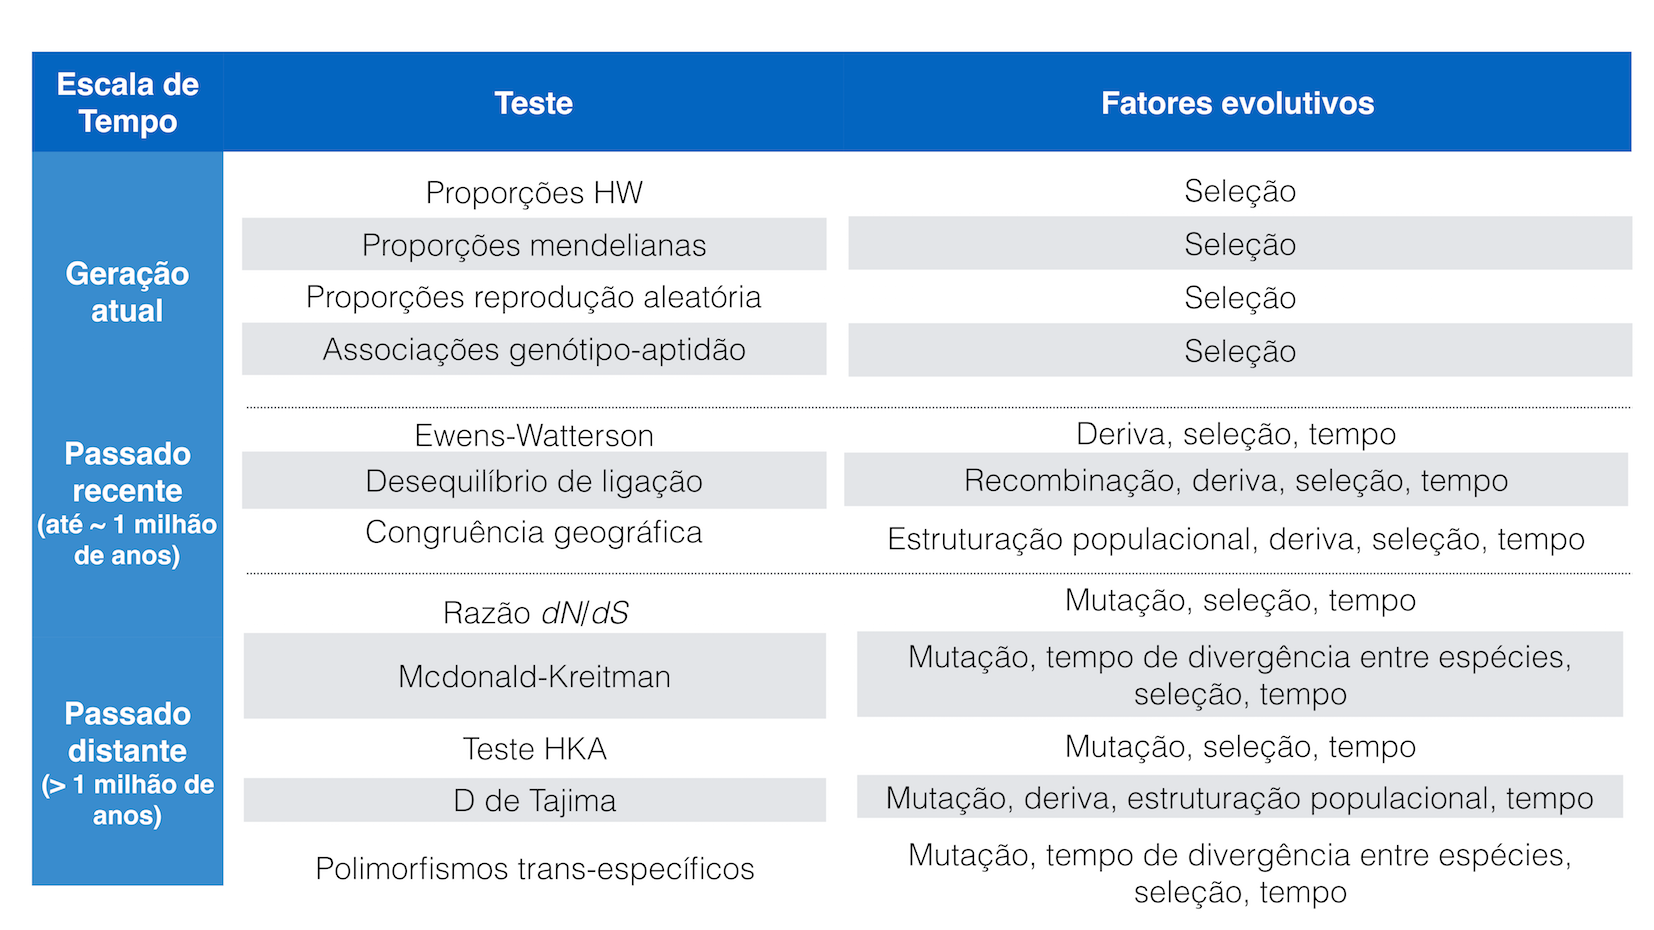
\includegraphics[width=\textwidth,keepaspectratio]{chap1_folder/Figures/hedrick_signatures_balsel_v2.png}
\caption{HW, Hardy-Weinberg, refere-se às proporções $p^2+2pq+q^2=1$ para os genótipos. Figura adaptada a partir de \textcite{Hedrick2012}. As assinaturas e os testes de neutralidade correspondentes são abordados no item \enquote{Assinaturas de seleção balanceadora}.}  %MELHORAR ESSA LEGENDA< EXPLICAR OS TESTES DE GERACAO ATUAL \nocite{Hedrick2012}
\label{fig:TestesBS}
\end{figure}
%%%%%%%%%%%%%%%%%%%%%%%%%%%%%%%%%%%%%%%%%%%%%%%%%%%%%%%%%%%%%%%%%%%%%%%%%%%%%%%%%%%%%%%%%%%%%%%%%%%%%%%%%%%%%%%%%%%%%%%%%%%%%%%%%%%%%%%%%%%%%%%%
%%%%%%%%%%%%%%%%%%%%%%%%%%%%%%%%%%%%%%%%%%%%%%%%%%%%%%%%%%%%%%%%%%%%%%%%%%%%%%%%%%%%%%%%%%%%%%%%%%%%%%%%%%%%%%%%%%%%%%%%%%%%%%%%%%%%%%%%%%%%%%%%
%%%%%%FIGURE%%%%%FIGURE%%FIGURE%%%%%%%%%FIGURE%%%%%FIGURE%%FIGURE%%%%%%%%%FIGURE%%%%%FIGURE%%FIGURE%%%%%%%%%FIGURE%%%%%FIGURE%%FIGURE%%%FIGURE%%

%%%%%%%%%%%%%%%%%%%%%%%%%%%%%%%%%%%%%%%%
\subsubsection{Seleção de curto prazo}
%%%%%%%%%%%%%%%%%%%%%%%%%%%%%%%%%%%%%%%%
    Em relação a eventos de seleção ocorridos no passado \enquote{recente} (até cerca de 1 milhão de anos atrás; \cite{Fu2013}), um dos primeiros testes do modelo neutro foi o de Ewens-Watterson (e.g. \cite{Watterson1978}), ou teste de homozigose da amostra (Figura ~\ref{fig:TestesBS}). Esse teste assume o modelo IAM (modelo de infinitos alelos\footnote{Um modelo que postula que cada novo alelo que surge em uma população é \enquote{novo} ou \enquote{único}, i.e, diferente de todos os que surgiram antes. Esse modelo foi proposto por \textcite{Kimura1964} em uma tentativa de estimar a proporção de loci homozigotos em uma população diploide finita.}), e que a população encontra-se em equilíbrio entre mutação e deriva. O teste relaciona a expectativa de número de loci homozigotos esperados em uma população em equilíbrio com aquela que de fato é observada. Uma deficiência de homozigose pode ser interpretada como indício de seleção balanceadora (i.e. os alelos segregam em frequências intermediárias, diminuindo a homozigose observada). Esse teste foi muito influente em estudos prévios à era genômica, mas hoje em dia é preterido por outros, que têm maior poder. %ask DM for ref here.

    Outros testes com poder para detectar assinaturas de eventos de seleção balanceadora compatíveis com essa escala de tempo olham: (a) a distribuição de frequências alélicas observada, comparando com aquela esperada sob o modelo neutro, (b) a variação genética e desequilíbrio de ligação\footnote{Uma medida que reflete se dois alelos em dois diferentes \emph{loci} coexistem de forma não-neutra em uma população. Alelos em desequilíbrio de ligação são encontrados mais frequentemente no mesmo haplótipo do que seria esperado se a recombinação ocorresse livremente entre eles (revisado em \cite{Cutter2013}).} em certas regiões genômicas com as observadas em regiões evoluindo de forma neutra, (c) a diferenciação geográfica observada em certos loci com aquelas encontradas para marcadores neutros \parencite{Hedrick2006,Hedrick2012,Mitchell-Olds2007} (Figura ~\ref{fig:TestesBS}). 
%  
%[Tem uma safra de estudos pré genômicos que você não menciona, que são
%aqueles baseados no teste de homozigose de neutralidade. Eles assumem o
%modelo de infinitos alelos e foram muito influentes, mas relativamente
%pouco conclusivos, devido ao seu baixo poder. Uma referência emblemática
%é a do Watterson: http://www.ncbi.nlm.nih.gov/pubmed/863245]
%tentei incluir isso acima, veja se está bom.

  
%  [Aqui vale o comentário anterior. Testes como o descrito no paper do
%  Watterson não são da geração presente, e usam um modelo mutacional do
%  tipo IAM (e não basedo em sequências). Então se você quiser ser
%  precisa valeria mencionar essa classe de testes]

%BDB: acho que consegui cobrir isso acima. Veja o que acha.
 
 
	A desvantagem de testes focados em desequilíbrio de ligação (Figura ~\ref{fig:TestesBS}) é que essa assinatura é essencialmente indistinguível daquela deixada por varreduras seletivas incompletas (seleção positiva). Uma outra assinatura que pode ser observada ao nível populacional é que diferentes subpopulações terão pouca diferenciação entre elas para loci-alvo de seleção balanceadora, dado que ela mantém variantes em frequências intermediárias em ambas as populações. Essa assinatura depende de uma congruência entre regimes seletivos entre os ambientes ocupados pelas duas populações e de ausência de adaptação local de uma ou mais subpopulações (Figura ~\ref{fig:TestesBS}). 
    
       Por outro lado, com a disponibilidade de dados de sequência, tornou-se possível investigar o efeito cumulativo da seleção ao longo de diversas gerações. O sinal de seleção no passado recente é gerado ou perdido ao longo de dezenas a milhares de gerações, dependendo da influência de deriva genética, fluxo gênico e recombinação \parencite{Hedrick2012}. 


\subsubsection{Seleção de longo prazo}

	O sinal de seleção que começou no passado distante e durou muito tempo\footnote{À qual nos referiremos como seleção balanceadora de longo prazo, SBLP, e em humanos corresponde a eventos que ocorreram há mais de um milhão de anos, ainda que possam ter persistido até recentemente (\cite{Fu2013}).} é determinado principalmente por mutação e seleção (Figura ~\ref{fig:TestesBS}), e geralmente leva de milhares a milhões de gerações para ser gerado. Quando persiste por milhares a milhões de gerações, a seleção balanceadora resulta não apenas na manutenção de maior quantidade de alelos nas populações (\cite{Andres2009}), mas também em uma maior persistência, ao longo do tempo, da diversidade alélica em relação à variação neutra (\cite{Richman2000}). Em outras palavras, em casos de seleção balanceadora de longo prazo, alelos segregando para um dado loco têm um TMRCA\footnote{\emph{Time to most recent common ancestor}, tempo de coalescência até o ancestral comum mais recente.} mais longo, o que implica em determinadas assinaturas genômicas: excesso de polimorfismos na região do sítio selecionado (pois haverá mais tempo para que mutações ocorram no haplótipo) e uma manutenção de tais polimorfismos por mais tempo que o esperado para uma mutação neutra, que acaba por ser fixada ou perdida após, em média, $4N$ gerações (onde $N$ é o tamanho da população).
%verificar se posso falar isso assim.
%
%%%%%%%%%%%%%%%%%%%%%%%%%%%%%%%%%%%%%%%%%%%%%%%%%%%%%%%%%%%%%%%%%%%%%%%%%%%%%%
\paragraph{Relação entre taxas de substituição não-sinônimas e sinônimas}%
%%%%%%%%%%%%%%%%%%%%%%%%%%%%%%%%%%%%%%%%%%%%%%%%%%%%%%%%%%%%%%%%%%%%%%%%%%%%%%
De acordo com a teoria neutra \parencite{Kimura1968,Kimura1983}, mutações capazes de alterar a função de uma proteína (mutações não-sinônimas) geralmente são deletérias e, portanto, alvo da seleção purificadora. Análises comparativas apontam que ao menos 38\% das mutações não-sinônimas sejam deletérias (\cite{Eyre-Walker1999}). Já as mutações sinônimas, que não alteram a sequência de aminoácidos da proteína, evoluiriam de forma neutra\footnote{Embora algumas mutações sinônimas possam ser alvo de seleção devido ao viés no uso de códons e uma parcela das mutações não-sinônimas ser neutra, a premissa é válida devido às proporções (e.g. \cite{Comeron2008}).}. A evolução adaptativa pode levar a um aumento da taxa de substituição de mutações não-sinônimas ($dN$), tornando-a mais alta do que a taxa de substituição sinônima ($dS$).
%

	Nesse sentido, a razão $dN/dS>1$ (ou $\omega>1$) é uma assinatura genética de seleção positiva \parencite{Gillespie1991,Nielsen2005}, mas também de seleção balanceadora (e.g. \cite{Bitarello2015}\footnote{Esta referência está disponibilizada no Apêndice A.4.}) (Figura ~\ref{fig:TestesBS}). Entretanto, o critério de $\omega > 1$ para considerar que genes estejam sob evolução adaptativa é muito conservador. Partindo da premissa de que a maior parte das mutações não-sinônimas é deletéria \parencite{Kimura1963,Kimura1968,Eyre-Walker1999}, o critério muitas vezes não é atendido quando genes inteiros são analisados. Isso ocorre porque geralmente apenas alguns códons estão sob seleção positiva ou balanceadora, enquanto a maior parte das mutações não-sinônimas são deletérias e, portanto, estão sob seleção purificadora\footnote{Essa ideia é indiretamente explorada no Capítulo 2.}. Por isso, há algum tempo convencionou-se analisar subconjuntos de códons em busca de seleção (e.g. \cite{Hughes1988,Hughes1989a,Bitarello2015}) ou através de modelos que estimam diferentes valores de $dN/dS$ para grupos de códons \parencite{Yang2002a, Bitarello2015}, tornando possível inferir quais deles evoluíram adaptativamente.
%%%%%%%%%%%%%%%%%%%%%%%%%%%%%%%%%%%%%%%%%%%%%%%%%%%%%%%%%%%%%%%%%%%%%%%%%
\paragraph{Espectro de frequências alélicas} 
Evidências de seleção do passado distante podem também ser baseadas na distribuição de frequência dos alelos de uma amostra, o espectro de frequências alélicas (SFS, \emph{site frequency spectrum}). O SFS é uma contagem do número de mutações que existem em uma frequência de $x_{i}=i/n$ para $i=1,2,...,n-1$ em uma amostra de tamanho $n$, onde $x$ é a frequência relativa de cada contagem. Em outras palavras, o SFS sumariza as frequências alélicas das várias mutações presentes em uma amostra (\cite{Nielsen2005}). Muitos testes estatísticos em genética de populações usam informação acerca da proporção de SNPs que são comuns ou raros, e acerca da frequência de alelos derivados e ancestrais, a fim de fazer inferências sobre a história demográfica e possíveis regimes seletivos. Um dos testes dentro dessa categoria é o \emph{D} de Tajima \parencite{tajima1989statistical,Mitchell-Olds2007} (Figura ~\ref{fig:TestesBS}). No Capítulo 1, nós propomos dois novos testes que exploram essa assinatura\footnote{As figuras 1 e 5 do Capítulo 1 mostram espectros de frequência alélica esquemático e de dados reais, respectivamente.}.

%[Eu acho que aqui caberia uma definição formal do que é um SFS. Ela está implícita na redação, mas acho que seria útil vê-la definida]
%BDB: done.

%%%%%%%%%%%%%%%%%%%%%%%%%%%%%%%%%%%%%%%%%%%%%%%%%%%%%%%%%%%%%%%%%%%%%%%%%


\paragraph{Relação entre níveis de polimorfismo e divergência\label{topico:poldiv}} 
Outros testes para seleção balanceadora nessa escala de tempo se baseiam em comparações entre os níveis de polimorfismo (observados dentro de uma espécie) e os níveis de divergência (entre duas espécies)\footnote{Ao longo do texto, e particularmente no Capítulo 1, refiro-me a substituições entre humanos e chimpanzés embora em princípio possa se tratar de substituições entre quaisquer duas espécies.}. Aqui inclui-se o teste Hudson-Kreitman-Aguadé, ou HKA \parencite{Hudson1987}, usado para testar predições do modelo neutro de evolução molecular. Um excesso de polimorfismo em relação a divergência pode ser interpretado como evidência de seleção balanceadora (Figura ~\ref{fig:TestesBS}).

	Uma versão modificada do teste HKA -- o teste de McDonald-Kreitman (MK) -- compara polimorfismos e divergência entre diferentes classes de mutação, como as substituições sinônimas e não-sinônimas \parencite{McDonald1991}. Nas situações em que há um excesso de divergência não-sinônima, temos um padrão consistente com seleção positiva (que fixa diferenças entre espécies e remove polimorfismos, explicando o padrão descrito). Já um excesso de polimorfismos não-sinônimos pode ser interpretado como uma assinatura de seleção balanceadora (Figura ~\ref{fig:TestesBS}). 
    Entretanto, conforme discutido por \textcite{Eyre-Walker2006}, essa estatística é muito sensível a mudanças de tamanho populacional, e mesmo aumentos modestos de $N_{e}$ podem criar evidências espúrias de evolução adaptativa. \textcite{Sella2009}, por sua vez, argumentam que uma das premissas mais problemáticas do teste MK é a de que a fração de novas mutações que é neutra, que é estimada a partir dos dados de polimorfismo de uma das espécies, tenha permanecido constante durante a história evolutiva das duas espécies sendo comparadas. A razão pela qual essa premissa é problemática é que uma história demográfica que resulta em uma população atual fora de equilíbrio torna essa premissa falsa quando a seleção é fraca, resultando em estimativas erradas de taxa de evolução adaptativa (por exemplo, \cite{Eyre-Walker2006,Fay2001,Nielsen2005,Sella2009}).
    

%DM[Para ser precisa, valeria um "mas veja Eyre-Waler naquele review dele na Trends e  Sella e tal, naquele artigo sobre pervasive selection) para dificuldades na interpretação desses testes, em particular no que se refere a efeitos da história demográfica e sua forma de itnerageir com a seleção natural]
%BDB: veja se tá bom.


%seria util ter aquela classica figura do tmepo de coalescencia, tipo no Bamshad & Wooding, e tambem no review da Aida.

\paragraph{Partilhamento de polimorfismos entre espécies} Finalmente, se um polimorfismo é mantido por seleção balanceadora por um tempo suficientemente longo, o mesmo polimorfismo pode ser encontrado em duas espécies-irmãs: um polimorfismo trans-específico \parencite{Hedrick2012,Klein1998} (Figura ~\ref{fig:TestesBS}). 

Se a possibilidade de que mutações idênticas tenham ocorrido independente nas duas espécies puder ser descartada -- por exemplo requirindo-se que mais de um polimorfismo seja compartilhado dentro de um haplótipo de tamanho reduzido (e.g. \cite{Leffler2013a,Teixeira2015}) -- , a outra possível explicação é que o polimorfismo seja neutro e mantido \enquote{ao acaso} nas duas espécies. Se o tempo de divergência entre as espécies é muito maior do que o tempo médio de coalescência intra-específica, essa alternativa tem baixíssima probabilidade. 

\textcite{Teixeira2015}, por exemplo, demonstraram que a probabilidade de um polimorfismo em humanos ser também um polimorfismo em chimpanzés e bonobos é da ordem de $10^{-10}$. Mesmo supondo independência entre todos os SNPs, considerando amostras de 20 indivíduos de cada espécie, a probabilidade de haver um polimorfismo partilhado é de $\sim 0.00005$, ou seja, praticamente zero. Portanto, embora essa assinatura seja extremamente convincente como evidência de seleção balanceadora de longo prazo, ela é bastante rara.  

%[Precisa de um link aqui para dizer que dependnedo do tempo de separação entre as espécies isso é extremamente pouco provável sob neutralidade, o que favore interepretações de que há seleção balanceadora]
%BDB: acho que ficou legal agora. veja.

% 
%%%%%%%%%%%%%%%%%%%%%%%%%%%%%%%%%%%%%%%%%%%%%%%%%%%%%%%%%%%%%%%%%%%%%%%%%%%%%%%%%%%%%%%%%%%%%%%%%%%%%%%%%%%%%%%%%%%%%%%%%%%%%%%%%%%%%%%%%%%%%%%%
%%%%%%%%%%%%%%%%%%%%%%%%%%%%%%%%%%%%%%%%%%%%%%%%%%%%%%%%%%%%%%%%%%%%%%%%%%%%%%%%%%%%%%%%%%%%%%%%%%%%%%%%%%%%%%%%%%%%%%%%%%%%%%%%%%%%%%%%%%%%%%%%

%%%%%%%%%%%%%%%%%%%%%%%%%%%%%%%%%%%%%%%%%%%%%%%%%%%%%%%%%%%%%%%%%%%%%%%%%%%%%%%%%%%%%%%%%%%%%%%%%%%%%%%%%%%%%%%%%%%%%%%%%%%%%%%%%%%%%%%%%%%%%%%%
%%%%%%%%%%%%%%%%%%%%%%%%%%%%%%%%%%%%%%%%%%%%%%%%%%%%%%%%%%%%%%%%%%%%%%%%%%%%%%%%%%%%%%%%%%%%%%%%%%%%%%%%%%%%%%%%%%%%%%%%%%%%%%%%%%%%%%%%%%%%%%%%
%%%%%%%%%%%%%%%%%%%%%%%%%%%%%%%%%%%%%%%%%%%%%%%%%%%%%%%%%%%%%%%%%%%%%%%%%%%%%%%%%%
\subsection{Seleção balanceadora no genoma humano} %%%%%%%%%%%%%%%%%%%%%%%%%%%%%%%
%%%%%%%%%%%%%%%%%%%%%%%%%%%%%%%%%%%%%%%%%%%%%%%%%%%%%%%%%%%%%%%%%%%%%%%%%%%%%%%%%%
\medskip
\begin{quotation}
\enquote{\emph{Balancing selection is not unique to the human lineage, nor is it the dominant force in shaping the human genome. It is, however, there and its effects are without dispute.}} (\cite{VallenderJohnson2008}) 
\end{quotation}
\medskip



%refrasear, ta identico ao Hedrick.
  
Embora diversos \emph{scans} genômicos tenham sido feitos com o intuito de localizar alvos de seleção positiva (revisado em \cite{Akey2009}), poucos trabalhos, comparativamente, buscaram localizar alvos de seleção balanceadora. Em parte isso é devido às dificuldades de detecção desse tipo de seleção em escala genômica \parencite{Andres2009}. A Figura~\ref{fig:AllScans} resume os estudos que buscaram por assinaturas de seleção balanceadora em humanos.

%DM[Figura ou tabela?]
%BDB: é um png, então eu disse que é figura porque nao da pra inserir figura num table float. acho que ta de boa, nao?

Até muito recentemente, não se havia estabelecido mais que alguns poucos casos de seleção balanceadora em humanos. Mesmo com o advento de dados de sequência pra diversos genes, poucos alvos foram propostos além dos genes HLA, do gene ABO e do gene da hemoglobina S (\cite{Allison1954,Kummerfeld2005,Bubb2006,Hughes1988,Segurel2013,}).

%%%%%%%%%%%%%%%%%%%%%%%%%%%%%%%%%%%%%%%%%%%%%%%%%%%%%%%%%%%%%%%%%%%%%%%%%%%%%%%%%%%%%%%%%%%%%%%%%%%%%%%%%%%%%%%%%%%%%%%%%%%%%%%%%%%%%%%%%%%%%%%%
%%%%%%%%%%%%%%%%%%%%%%%%%%%%%%%%%%%%%%%%%%%%%%%%%%%%%%%%%%%%%%%%%%%%%%%%%%%%%%%%%%%%%%%%%%%%%%%%%%%%%%%%%%%%%%%%%%%%%%%%%%%%%%%%%%%%%%%%%%%%%%%%
%%%%%%FIGURE%%%%%FIGURE%%FIGURE%%%%%%%%%FIGURE%%%%%FIGURE%%FIGURE%%%%%%%%%FIGURE%%%%%FIGURE%%FIGURE%%%%%%%%%FIGURE%%%%%FIGURE%%FIGURE%%%FIGURE%%
%%%%%%%%%%%%%%%%%%%%%%%%%%%%%%%%%%%%%%%%%%%%%%%%%%%%%%%%%%%%%%%%%%%%%%%%%%%%%%%%%%%%%%%%%%%%%%%%%%%%%%%%%%%%%%%%%%%%%%%%%%%%%%%%%%%%%%%%%%%%%%%%
%%%%%%%%%%%%%%%%%%%%%%%%%%%%%%%%%%%%%%%%%%%%%%%%%%%%%%%%%%%%%%%%%%%%%%%%%%%%%%%%%%%%%%%%%%%%%%%%%%%%%%%%%%%%%%%%%%%%%%%%%%%%%%%%%%%%%%%%%%%%%%%%
\begin{figure}[ht]
\centering
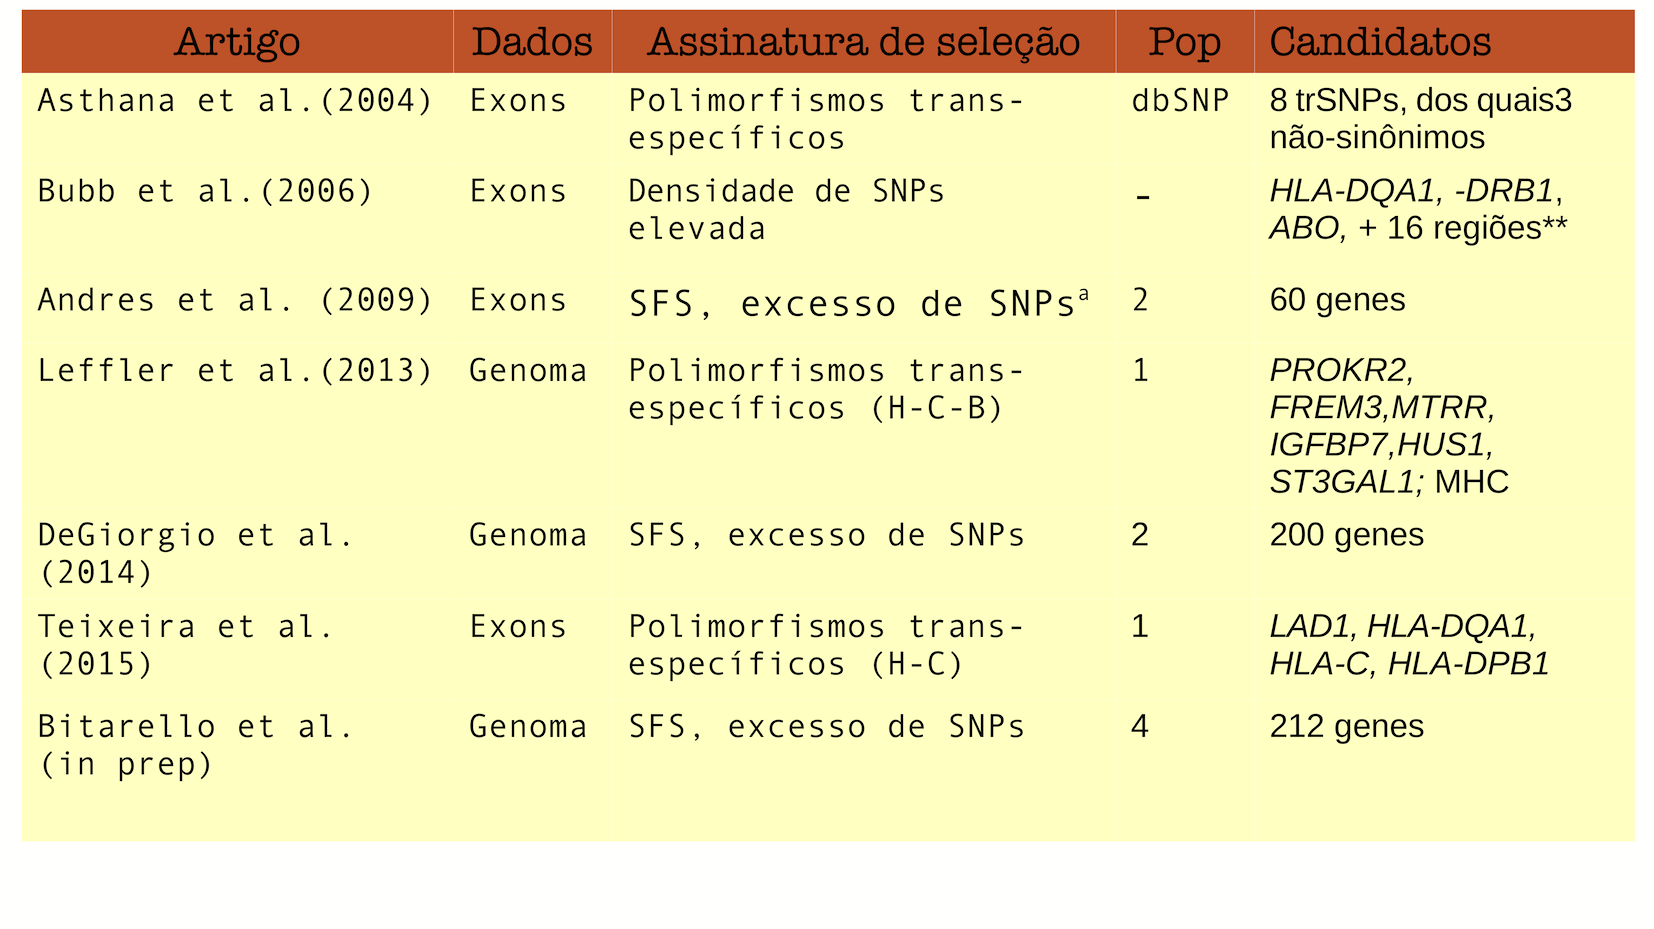
\includegraphics[width=0.8\textwidth]{chap1_folder/Figures/all_scans_v2.png}
\caption{Resumo dos estudos que buscaram assinaturas de seleção balanceadora de longo prazo em humanos. SFS, espectro de frequências alélicas; dbSNP, banco de dados de SNP, indica que o estudo não usou informações de frequências de SNPs estimadas para populações individuais, mas de um banco de dados comum; trSNPs, SNPs trans-específicos entre (H-C) humano-chimpanzé ou (H-C-B) humano, chimpanzé, bonobo. a, excesso de SNPs em relação a sítios divergentes entre humanos e chimpanzé, uma assinatura de seleção balanceadora. ** apesar de que eles encontram 16 regiões com alta diversidade genética além de genes HLA e o gene ABO, os autores as descartam como reais candidatas pois não possuem evidência de polimorfismo trans-específico, o que é um critério muito rigoroso (ver \enquote{Assinaturas de seleção balanceadora}.)}
\label{fig:AllScans}
\end{figure}
%%%%%%%%%%%%%%%%%%%%%%%%%%%%%%%%%%%%%%%%%%%%%%%%%%%%%%%%%%%%%%%%%%%%%%%%%%%%%%%%%%%%%%%%%%%%%%%%%%%%%%%%%%%%%%%%%%%%%%%%%%%%%%%%%%%%%%%%%%%%%%%%
%%%%%%%%%%%%%%%%%%%%%%%%%%%%%%%%%%%%%%%%%%%%%%%%%%%%%%%%%%%%%%%%%%%%%%%%%%%%%%%%%%%%%%%%%%%%%%%%%%%%%%%%%%%%%%%%%%%%%%%%%%%%%%%%%%%%%%%%%%%%%%%%
%%%%%%FIGURE%%%%%FIGURE%%FIGURE%%%%%%%%%FIGURE%%%%%FIGURE%%FIGURE%%%%%%%%%FIGURE%%%%%FIGURE%%FIGURE%%%%%%%%%FIGURE%%%%%FIGURE%%FIGURE%%%FIGURE%%
%%%%%%%%%%%%%%%%%%%%%%%%%%%%%%%%%%%%%%%%%%%%%%%%%%%%%%%%%%%%%%%%%%%%%%%%%%%%%%%%%%%%%%%%%%%%%%%%%%%%%%%%%%%%%%%%%%%%%%%%%%%%%%%%%%%%%%%%%%%%%%%%
%%%%%%%%%%%%%%%%%%%%%%%%%%%%%%%%%%%%%%%%%%%%%%%%%%%%%%%%%%%%%%%%%%%%%%%%%%%%%%%%%%%%%%%%%%%%%%%%%%%%%%%%%%%%%%%%%%%%%%%%%%%%%%%%%%%%%%%%%%%%%%%%


O primeiro estudo em escala genômica que identificou novas assinaturas de seleção balanceadora em humanos foi o de \textcite{Andres2009}. Nele, foi feito um \emph{scan} para genes sob seleção balanceadora de longo prazo (SBLP) no genoma humano. O \emph{scan} de Andrés et al. utilizou uma base de dados de exoma consistindo de 13.400 genes de duas populações humanas (19 norte-americanos com ancestralidade europeia e 20 norte-americanos com ancestralidade africana). O método consistiu em contrastar padrões de polimorfismo em cada gene com o resto do genoma e com as expectativas neutras, obtidas através de simulações parametrizadas pelos próprios dados de sequenciamento. O método buscava genes com duas assinaturas de SBLP: excesso de variantes em frequências intermediárias e excesso de sítios polimórficos em humanos (em relação a substituições entre humanos e chimpanzés)\footnote{Ambas as assinaturas servem de base para testes discutidos na seção anterior.}.

Apenas genes extremos em relação a ambas as assinaturas, i.e, altamente significativos para dois testes independentes, foram considerados como candidatos. Apesar do baixo poder estatístico deste tipo de abordagem \parencite{Fijarczyk2015}, ela tem poucos falsos positivos. Foram encontrados 60 genes com assinaturas de SBLP, muitos deles envolvidos com a imunidade, mas não restritos aos exemplos clássicos até então descritos \parencite{Key2014b}.

Foi observado que a maior parte dos loci sob seleção balanceadora eram compartilhados entre as duas populações, com poucas exceções : quatro genes com evidência de seleção balanceadora apenas nos americanos com ascendência africana e nove apenas nos americanos com ascendência europeia.

A ausência de sequências flanqueadoras não-codificadoras, intergênicas e intrônicas nas bases de dados desse estudo tem duas consequências: primeiro, os efeitos da seleção balanceadora sobre regiões ligadas a loci sob seleção não puderam ser quantificados; segundo, alvos de seleção balanceadora em regiões não-codificadoras não puderam ser detectadas.

Mais recentemente, \textcite{DeGiorgio2014} desenvolveram dois novos testes para a identificação de padrões locais de diversidade esperados em posições ligadas a um polimorfismo balanceado (T1 e T2) para a identificação e usaram esses métodos em dados genômicos de duas populações (YRI, Yoruba, uma população africana e CEU, uma população de norte-americanos do Utah com ascendência norte-europeia). Eles identificaram 200 genes candidatos (Figura ~\ref{fig:AllScans}) -- alguns deles conhecidos (e.g. \cite{Andres2009}), e outros novos \parencite{Key2014b}. 



Três importantes limitações destes trabalhos são que: (1) apesar de o trabalho mostrar que os métodos T1 e T2 têm poder elevado sob modelos simples, os autores não exploram modelos demográficos humanos (e.g. \cite{Gravel2011}); (2) os 200 genes reportados provêm de uma lista dos \enquote{100 genes mais extremos} para cada teste e população, mas não foi estabelecido um critério para que 100 genes fossem reportados; portanto, esse trabalho, apesar de inquestionavelmente contribuir muito para o conhecimento acumulado de regiões do genoma humano que possuem assinaturas de SBLP, não fornece uma estimativa aproximada do quão frequente ela pode ser no genoma humano; (3) apesar de os autores terem usado dados de genoma completo, eles reportam como alvos apenas genes codificadores de proteínas, e não exploram ou reportam regiões genômicas candidatas que estão fora dos limites gênicos.


%O scan de Andrés et al., juntamente com abordagens de genes candidatos que revelaram seleção balanceadora (por exemplo, Cagliani et al., 2010; Meyer et al., 2006) e estudos teóricos indicando a provável importância da seleção balanceadora na evolução adaptativa (e.g. Sellis et al., 2011) renovaram o interesse acerca desse tipo de seleção, e motivam o presente estudo.

Finalmente, dois estudos em escala genômica buscaram por polimorfismos partilhados entre humanos e outras espécies: trata-se da assinatura mais extrema de SBLP,  pois requer a manutenção de polimorfismos por milhões de anos. \textcite{Leffler2013a} olharam o genoma completo de humanos e chimpanzés e buscaram por polimorfismos compartilhados, encontrando seis genes com forte evidência de polimorfismos balanceados compartilhados (Figura ~\ref{fig:AllScans}), e \textcite{Teixeira2015} olharam os éxons de humanos, chimpanzés e bonobos, encontrando forte evidência de polimorfismo balanceado partilhado entre as três espécies no gene \emph{LAD1}, além de alguns genes HLA (Figura ~\ref{fig:AllScans}).
%%

Eventos de seleção balanceadora de curto e longo prazo deixam assinaturas genômicas que não permitem diferenciar entre os mecanismos de seleção balanceadora expostos anteriormente. Além disso, um sinal de seleção de longo prazo não significa que a seleção tenha perdurado até o passado recente ou até a geração atual. Vê-se, portanto, que definir escalas de tempo dos regimes seletivos é importante tanto no sentido de determinar quais as ferramentas adequadas, quanto no grau de resolução que se pode alcançar. 
%%melhorar isso

%DM[A frase inicial não flui tão bem, revise please. Sugestão: separe conceitualmente a ocorrência da seleção e sua detecção via testes. Na frase assina os eventos e assinaturas se misturam, então redigir de uma forma que mostre que assinaturas relevelam eventos ou que eventos podem deixar assinaturas ficará melhor]
%BDB: checar, plis?


Por si só as análises de genética de populações acima descritas são capazes de identificar genes que evoluíram de forma não-neutra durante milhares ou até milhões de gerações. Essa é o tipo de investigação proposta no Capítulo 1, a fim de melhor compreender o impacto da seleção balanceadora de longo prazo no genoma humano. Tal tipo de investigação não fornece, todavia, informação conclusiva acerca do caráter fenotípico que foi alvo de seleção \parencite{Mitchell-Olds2007}. Trata-se de um desafio em andamento na genômica de populações, e que será discutido no item Discussão e Considerações Finais (Página ~\pageref{chap:conclusions}).

%%%%%%%%%%%%%%%%%%%%%%%%%%%%%%%%%%%%%%%%%%%%%%%%%%%%%%%%%%%%%%%%%%%%%%%%%%%%%%%%%%%%%%%%%%%%%%%%%%%%%%%%%%%%%%%%%%%%%%%%%%%%%%%%%%%%%%%%%%%%%%%%%%%%%%%%%%%%%%%%%%%%%%%%%%%%%%%%%%%%%%%%%%%%%%%%%%%%%%%%%%%%%%%%%%%%%%%%%%%%%%%%%%%%%%%%%%%%%%%%%%%%%%%%%%%%%%%%%%%%%%%%%%%%%%%%%%%%%%%%%%%%%%%%
%%%%%%%%%%%%%%%%%%%%%%%%%%%%%%%%%%%%%%%%%%%%%%%%%%%%%%%%%%%%%%%%%%%%%%%%%%%%%%%%%%%%%%%%%%%%%%%%%%%%%%%%%%%%%%%%%%%%%%%%%%%%%%%%%%%%%%%%%%%%%%%%%%%%%%%%%%%%%%%%%%%%%%%%%%%%%%%%%%%%%%%%%%%%%%%%%%%%%%%%%%%%%%%%%%%%%%%%%%%%%%%%%%%%%%%%%%%%%%%%%%%%%%%%%%%%%%%%%%%%%%%%%%%%%%%%%%%%%%%%%%%%%%%%%%%%%%%%%%%%%%%%%%%%%%%%%%%%%%%%%%%%%%%%%%%%%%%%%%%%%%%%%%%%%%%%%%%%%%%%%%%%%%%%%%%%%%%%%%%%%%%%%%%%%%%%%%%%%%%%%%%%%%%%%%%%%%%%%%%%%%%%%%%%%%%%%%%%%%%%%%%%%%%%%%%%%%%%%%%%%%%%%%%%%%%%%%%%%%%%%%%%%%%%%%%%%%%%%%%%%%%%%%%%%%%%%%%%%%%%%%%%%%%%%%%%%%%%%%%%%%%%%%%%%%%%%%%%%%%%%%%%%%%%%%%%%%%%
%%% TERCEIRA PARTE DA INTRODUCAO %%%%%%%%%%%%%%%%%%%%%%
%%%%%%%%%%%%%%%%%%%%%%%%%%%%%%%%%%%%%%%%%%%%%%%%%%%%%%%%%%%%%%%%%%%%%%%%%%%%%%%%%%%%%%%%%%%%%%%%%%%%%%%%%%%%%%%%%%%%%%%%%%%%%%%%%%%%%%%%%%%%%%%%%%%%%%%%%%%%%%%%%%%%%%%%%%%%%%%%%%%%%%%%%%%%%%%%%%%%%%%%%%%%%%%%%%%%%%%%%%%%%%%%%%%%%%%%%%%%%%%%%%%%%%%%%%%%%%%%%%%%%%%%%%%%%%%%%%%%%%%%%%%%%%%%%%%%%%%%%%%%%%%%%%%%%%%%%%%%%%%%%%%%%%%%%%%%%%%%%%%%%%%%%%%%%%%%%%%%%%%%%%%%%%%%%%%%%%%%%%%%%%%%%%%%%%%%%%%%%%%%%%%%%%%%%%%%%%%%%%%%%%%%%%%%%%%%
\section{Carga genética induzida por seleção balanceadora}  

%%%%%%%%%%%%%%%%%%%%%%%%%%%%%%%%%%%%%%%%%%%%%%%%%%%%%%%%%%%%%%%%%%%%
%opção
%\section{Mutações deletérias em humanos}

\begin{quotation}
\enquote{\emph{Hence there must be a far greater number of different kinds of ailments whose characteristics are traceable to genetic changes of natural origin than there are different kinds of infectious diseases. This general reasoning does not in itself give us much idea, however, of the actual frequencies with which these mutational disorders occur in populations. For this it is necessary to turn to quantitative studies.}} (\cite{Muller1950})  %decide if there is a better opening citation for this part.
\end{quotation}

%another option "linked genes will on the average interfere with each other’s fixation by increasing the %variance of off spring number and thereby decreasing the effectiveness of selection. If there is free %recombination, the organism will largely avoid this effect" (Felsenstein, 1974, defining HR-effect)

Como vimos, os polimorfismos de sequência podem estar evoluindo de forma neutra (provavelmente a grande maioria deles), mas podem também representar estados transientes de variantes genéticas rumo à eliminação por serem deletérias, ou rumo à fixação por serem vantajosas \parencite{Hudson1987,Mitchell-Olds2007,Sellis2011a}. Finalmente, uma certa quantidade desses polimorfismos é mantida em populações individuais por seleção balanceadora ou ao longo de toda a distribuição da espécie, por adaptação local\footnote{Situação na qual genótipos de diferentes populações têm aptidão maior em seus ambientes de origem, devido a seleção natural histórica na região.} (revisado em \cite{Mitchell-Olds2007}).

Estudos genômicos têm documentado grandes quantidades de polimorfismos, e tem-se feito muito progresso no sentido de compreender quais processos evolutivos moldaram tal variação (revisado em \cite{Mitchell-Olds2007}). Para um geneticista evolutivo, detectar possíveis alvos de seleção natural no genoma é fundamental. Primeiramente, padrões compatíveis com um cenário de evolução adaptativa (seleção positiva ou balanceadora) devem ser buscados. Um caminho são as assinaturas de seleção e os testes de neutralidade, vistos anteriormente. Uma vez detectadas as regiões de interesse, é necessário investigar se há base biológica para sustentar que tais padrões de fato resultem de seleção. Finalmente, pode-se investigar se a seleção sobre um dado loco no genoma tem consequências deletérias sobre regiões vizinhas.

A existência de assinaturas de seleção positiva ou balanceadora indica que pode ter havido adaptação para algum traço (aquele relacionado à pressão seletiva), mas a consequência da pressão seletiva pode incluir também mudanças que causam má-adaptação, em função de mudanças que ocorrem em outras regiões do mesmo gene que está sendo selecionado, ou mesmo em regiões não codificadoras  -- porém funcionais -- adjacentes.

%%%%%%%%%%%%%%%%%%%%%%%%%%%%%%
\subsection{Carga genética}%%%
%%%%%%%%%%%%%%%%%%%%%%%%%%%%%%
%

	A compreensão da base genética da adaptação requer a definição de “carga genética”. O conceito foi discutido pela primeira vez por \textcite{Haldane1937}, sendo posteriormente elaborado por \textcite{Muller1950}. A ideia central é que uma população fica aquém de sua aptidão máxima por dois motivos: (1) a ocorrência de mutações deletérias recorrentes (carga mutacional) e; (2) a produção de homozigotos menos aptos, nas situações em que os heterozigotos são o genótipo mais apto (carga segregacional). Esse decréscimo na aptidão máxima de uma população é a carga genética.
%

Embora as mutações deletérias incorram em um custo de aptidão, elas nem sempre são removidas da população de forma eficiente. É ainda mais difícil remover mutações deletérias de populações pequenas (baixos valores de $N_{e}$\footnote{Tamanho populacional efetivo: reflete o tamanho de uma população idealizada que estaria sujeita à deriva da mesma forma que a população de fato. O $N_{e}$ pode ser menor que o tamanho real da população devido a vários fatores, incluindo variância no sucesso reprodutivo, uma história demográfica com gargalos genéticos (reduções extremas de tamanho populacional, seguida de uma expansão a partir de uma amostra da população original) e endogamia (revisado em \cite{Cutter2013}).}), e seu acúmulo pode levar a reduções no tamanho populacional e, em última instância, à extinção (\cite{Chun2011}).
%

No âmbito da evolução molecular, a maior parte das mutações \emph{não} são adaptativas, piorando (mutações mal-adaptativas) ou não interferindo (neutras) no grau de adaptação dos caráteres ao ambiente \parencite{Orr1998}. A eficácia de remoção de variantes deletérias de uma população depende de vários fatores: mutação (que cria novas variantes deletérias constantemente), dominância (que influencia o quanto a mutação é \enquote{visível} para a seleção) (e.g. \cite{Sellis2011a}), demografia e ligação \parencite{Gravel2016}.  

Além disso, uma situação de má-adaptação de uma população pode ser causada por falta de variação genotípica segregante para responder à seleção. Deriva genética e endogamia, por exemplo, removem as populações de seus picos adaptativos e podem levar à má-adaptação fenotípica \parencite{Crespi2000}. A pleiotropia\footnote{Fenômeno em que um gene afeta múltiplos caracteres, considerado o modo quase universal de atuação gênica.} pode resultar em populações mal-adaptadas pois  a otimização conjunta de muitos caracteres é inviável \parencite{Charlesworth2010,Crespi2000}. Finalmente, a migração entre populações de indivíduos que se adaptaram em diferentes subpopulações pode também levar à má-adaptação \parencite{Charlesworth2010,Crespi2000}. %check these refs
%
%obsolete%
%No caso das substituições gênicas, o grau de adaptação e de má-adaptação pode ser quantificado como a “carga de atraso” (\emph{lag load}\footnote{Também chamada de \emph{substitutional lag}, ou carga substitucional.}). Esse terceiro tipo de carga genética (Maynard Smith, 1976) é o grau em que a aptidão do fenótipo atual está ”defasada” em
%relação ao genótipo ótimo de um ambiente modificado. Para Maynard Smith, “taxa de evolução” nada mais é do que a taxa de mudanças adaptativas, que depende da carga de atraso, do tamanho populacional efetivo, da taxa de mutação por loco e da vantagem seletiva por mutação favorável\footnote{Nesse sentido, uma substituição em um alelo neutro não constituiria “evolução”, o que diferencia a concepção evolutiva de Maynard Smith daquela da maior parte dos biólogos evolucionistas posteriores, que incorporaram a ideia de que a maior parte da evolução ocorre em função da deriva.}. 

 

A má-adaptação pode, ainda resultar de pressões seletivas para a adaptação em sítios ligados, que discutirei em maior detalhes abaixo. Nesse sentido, seja em termos fenotípicos, seja em termos genéticos (acúmulo de mutações deletérias), o termo má-adaptação alude a um “custo adaptativo” com o qual as populações têm que arcar em função de estarem evoluindo sob determinadas pressões seletivas.


%%%%%%%%%%%%%%%%%%%%%%%%%%%%%%%%%%%%%%%%%%%%%%%%%%%%%%%%%%%%
%%%%%%%%%%%%%%%%%%%%%%%%%%%%%%%%%%%%%%%%%%%%%%%%%%%%%%%%%%%%
\subsubsection{Efeitos de ligação sobre polimorfismos neutros}
%%%%%%%%%%%%%%%%%%%%%%%%%%%%%%%%%%%%%%%%%%%%%%%%%%%%%%%%%%%%
%%%%%%%%%%%%%%%%%%%%%%%%%%%%%%%%%%%%%%%%%%%%%%%%%%%%%%%%%%%%

A última década documentou uma explosão de estudos sobre a prevalência e efeito da seleção natural, em particular no genoma da nossa espécie. Um dos achados mais marcantes foi o fato de haver uma proporção relativamente grande de mudanças entre humanos e chimpanzés que resultam da seleção natural. Por exemplo, alguns estudos mostraram que até 10\% das substituições que carregamos resultam de seleção positiva (\cite{Bustamante2005,Fay2001}), uma fração muito maior do que seria esperado por um neutralista (revisado em \cite{Eyre-Walker2006}). Esses resultados foram obtidos usando uma abordagem que contrasta o grau de polimorfismo e divergência entre humanos e primatas\footnote{Conforme discutido na página ~\pageref{topico:poldiv} e na Figura ~\ref{fig:TestesBS}.}, e revelou que há mais diferenças fixas não-sinônimas entre as duas espécies do que seria esperado sob neutralidade -- diferenças essas que são explicáveis se supusermos que a seleção fixou mutações vantajosas diferentes entre as linhagens de humanos e chimpanzés (revisado em \cite{Eyre-Walker2006}).

É esperado que a seleção natural deixe assinaturas específicas sobre os padrões de variação neutra intimamente ligados ao sítio com a mutação vantajosa. Essa ideia é a base dos métodos de genética molecular de populações que buscam por adaptações no genoma humano \parencite{Kreitman2004}. Essa propriedade é crucial para que testes de neutralidade tenham poder para detectar regiões com assinaturas de seleção, ainda que o sítio selecionado seja apenas um (revisado em \cite{Charlesworth2006}). A informação genética em escala genômica permite também fazer inferências sobre consequências da seleção natural sobre regiões do genoma fisicamente próximas aos genes ou regiões genômicas selecionados(as). 


Existe também uma bem-documentada correlação positiva entre taxas de recombinação e níveis de polimorfismo em \emph{Drosophila} \parencite{Zhang2005} e em humanos \parencite{Hellmann2003}. Essa correlação é consistente com a ideia de que a seleção positiva ocorre em diversos locais do genoma, e quando afeta um gene numa região de baixa recombinação, \enquote{arrasta} com ele um uma parte do cromossomo (isto é, promove um evento de carona genética), que tem como consequência a perda da variação naquela região do genoma. Nesse processo, a variação neutra em sítios ligados é reduzida. E quanto menor for a taxa de recombinação na região, mais pronunciada será a perda de diversidade.

Estas varreduras seletivas\footnote{Fenômeno em que uma mutação recém-surgida e altamente adaptativa sobe rapidamente de frequência na população.} levam a uma queda de diversidade em torno do sítio selecionado, que, com o passar do tempo, vai progressivamente aumentado na medida em que aumenta a distância entre o sítio neutro e o sítio-alvo. O tamanho da área vizinha que perderá polimorfismos neutros depende da intensidade da seleção, da taxa de mutação e da taxa de recombinação (revisado em \cite{Bamshad2003}). Sabe-se hoje que a seleção positiva em humanos afeta bastante os sítios neutros próximos ao sítio selecionado, reduzindo em 6\% seu nível de polimorfismo ao longo de todo o genoma, e 11\% na porção codificadora de proteínas do genoma \parencite{Cai2009}. 

%[Rever a frase pois o trecho "e parece ser..." não está fluindo tão bem. Que tal. "...é reduzida, deixando uma assinatura identificável que, no caso do genoma humano, parece evidenciar que a remoção de variação devido à seleção em genes fisicamente próximos é um processo importante...". Mas repare que o resultado de redução em 6\% acima já tratava extamente disso. Então veja se dá para sintetizar aquele conteúdo com esse, pois o "força substancial" daqui é justamente aquele número que você havia dito acima]
%BDB: done.


Analogamente, a seleção balanceadora de longo prazo também afeta sítios neutros vizinhos \parencite{Charlesworth2006}. Por aumentar o tempo de coalescência, a seleção balanceadora leva a um aumento de diversidade em torno do sítio selecionado, além de mudar o formato do espectro de frequências alélicas local (SFS), que passa a ter um excesso de alelos segregando em frequências próximas à do polimorfismo balanceado (\cite{Andres2009,Andres2011,Bamshad2003,Charlesworth2006}). 

Entretanto, ao contrário das varreduras seletivas, que envolvem altos coeficientes seletivos e diminuem a diversidade neutra em relativamente poucas gerações, gerando assinaturas que se estendem por longos trechos do cromossomo (\cite{Bamshad2003}), a seleção balanceadora de longo prazo, por envolver escalas de tempo de milhares a milhões de anos, gera assinaturas em curtos segmentos em torno do polimorfismo balanceado\footnote{Uma propriedade que é explorada quando avaliamos o poder de nossas estatísticas no Capítulo 1.}. Isso ocorre porque, ao longo de muitas gerações, a recombinação tem a oportunidade de ir "quebrando" a ligação entre o polimorfismo balanceado e os sítios neutros vizinhos (\cite{Andres2011,Charlesworth2006}), assim reduzindo o efeito de ligação a segmentos curtos do cromossomo. 
	
%Review by Cutter and Payseus (2015)

%"Disease consequences of human adaptation" (Fay)

%%%%%%%%%%%%%%%%%%%%%%%%%%%%%%%%%%%%%%%%%%%%%%%%%%%%%%%%%%%%
%%%%%%%%%%%%%%%%%%%%%%%%%%%%%%%%%%%%%%%%%%%%%%%%%%%%%%%%%%%%

\subsubsection{Efeitos de ligação sobre polimorfismos não-neutros}
%%%%%%%%%%%%%%%%%%%%%%%%%%%%%%%%%%%%%%%%%%%%%%%%%%%%%%%%%%%%
%%%%%%%%%%%%%%%%%%%%%%%%%%%%%%%%%%%%%%%%%%%%%%%%%%%%%%%%%%%%

Existem dois modos através dos quais a seleção sobre um traço interfere sobre a seleção sobre outros traços. O primeiro se dá em condições em que um gene tem funções pleiotrópicas. Seleção positiva ou balanceadora pressupõe adaptação para algum traço (aquele relacionado à pressão seletiva), mas a consequência da pressão seletiva em termos de fixação de mutações pode não ser uma adaptação para todas as possíveis funções que exerce. Nesse caso, o “subproduto” seria uma má-adaptação. Como exemplo, temos os genes HLA, que estão relacionados à resposta imune em humanos e têm fortes evidências de seleção positiva e balanceadora. Por outro lado, muitas doenças inflamatórias e autoimunes também estão relacionadas aos genes de HLA \parencite{Becker1998}.

O segundo modo ocorre quando o sítio selecionado interfere sobre o destino de mutações não-neutras em sítios ligados geneticamente\footnote{Ver Figura 1 do Capítulo 2 na página ~\pageref{fig:schema}.}. A seleção natural não atua independentemente sobre locos ligados e, sendo assim, sua eficiência está diretamente relacionada à taxa de recombinação (\cite{Hill2009,Comeron2008}). A ligação entre sítios reduz a eficácia da seleção natural em populações finitas (\cite{Hill2009,Comeron2008}). Mantendo-se as outras variáveis constantes, espera-se que o grau de interferência entre alelos selecionados varie entre regiões com diferentes taxas de recombinação, potencialmente levando a mudanças nas taxas de evolução\footnote{\emph{Hill-Robertson Effect} é o nome dado a essa interferência (\cite{Hill2009,Comeron2008}).}. Regiões de baixa recombinação estariam sujeitas a efeitos mais pronunciados de Hill-Robertson, dado que a baixa recombinação reduz a independência entre os sítios, aumentando o efeito relativo da deriva sobre a região -- o que equivale a uma redução do $N_{e}$ local (\cite{Maynard-Smith1974,Comeron2008}). %preciso ler esse paper original do HRE


%[Esse não é um efeito de ligação e vem logo depois da introdução do HRI, o que tira o foco. Você pode começar dizendo que há dois modos como a seleção sobre um traço intefere com a de outros. O primeiro se dá nessas condições em que o gene tem funções pleiotrópicas. A segunda é o caso em que a seleção num gene afeta a frequência de variantes em outros, como ocorre nos casos de carona genética, ou HRI.]
%BDB: done, checar se ficou bom.



Diante da informação de que substituições adaptativas (fixadas por seleção positiva) são relativamente comuns, tornou-se importante investigar a forma como esses eventos influenciam a atuação da seleção natural em regiões adjacentes do genoma. As trajetórias até a fixação das variantes neutras ligadas a variantes vantajosas permanecem inalteradas -- dado que a probabilidade de uma mutação vantajosa carregar consigo uma mutação neutra é diretamente proporcional à frequência do alelo na população (\cite{Walsh1988,Chun2011,Comeron2008,Harris2010,Charlesworth2012}). Entretanto, mutações levemente deletérias, quando ligadas geneticamente a variantes vantajosas, terão probabilidade de fixação maior do que a esperada sob o modelo neutro (\cite{Lynch2007}).


%obsolete
%Rice (1987) sugere que os eventos de carona genética transformam a carga mutacional "dispersa" (várias mutações deletérias espalhadas pelo genoma) em uma carga "altamente localizada" (uma substituição deletéria), resultante do efeito carona. Ou seja, a carona opera sobre as mutações e, dessa forma, pode mudar a forma como a carga mutacional se manifesta. Em conjunto, esses resultados mostram que seleção positiva, fixando mutações vantajosas, é relativamente comum e é um mecanismo importante para explicar aspectos globais da organização do nosso genoma. Entretanto, estudos recentes têm argumentado que a quantidade de sítios sob seleção detectados pelas análises baseadas em comparações de polimorfismo e divergência supera o número de regiões do genoma com baixa variação, que seriam produtos de varreduras seletivas. 



O efeito da seleção positiva sobre regiões ligadas em \emph{Drosophila} foi investigado por \textcite{Betancourt2002}, que verificaram que os genes de evolução adaptativa lenta (sujeitos principalmente à seleção purificadora) se concentram principalmente nas regiões de baixa recombinação. Além disso, foi encontrada uma correlação negativa significativa entre a taxa de evolução (medida em termos de $dN$) e a proporção de uso de códons ótimos\footnote{Diferentes sítios sinônimos são seletivamente diferentes, uma vez que certos códons (ditos “ótimos”) são utilizados mais frequentemente que outros, possivelmente em função de eficiência e precisão da tradução \parencite{Betancourt2002}.}. Os autores descartaram a possibilidade de restrição seletiva relaxada; eles concluem que a causa para essa correlação é a interferência do sítio codificador sobre o fraco coeficiente seletivo para uso ótimo de códons em sítios vizinhos fortemente ligados.

A conclusão geral é que, ao menos em \emph{Drosophila}, parece haver uma “hierarquia de pressões seletivas”: a seleção contra mutações deletérias é mais forte do que a seleção sobre mutações não-sinônimas vantajosas, que por sua vez é maior do que a seleção para códons ótimos. O que não significa, conforme os próprios autores salientam, que o efeito cumulativo de muitos códons subótimos seja negligenciável. 

Além disso, foi demonstrado que a seleção direcional forte (positiva ou negativa) é capaz de gerar um aumento da proporção de variantes deletérias segregando em regiões adjacentes àquelas que foram alvo da seleção direcional em humanos \parencite{Chun2011}. Assim como os \emph{scans} genômicos para seleção balanceadora são muito menos abundantes que aqueles para seleção positiva, o mesmo ocorre em relação ao acúmulo de deletérias: até o momento, nenhum estudo investigou especificamente o impacto que a seleção balanceadora tem sobre o acúmulo de variantes deletérias em sítios na vizinhança do polimorfismo balanceado. 

Existe evidência de que genes na vizinhança dos genes HLA têm um excesso de variantes potencialmente deletérias \parencite{Mendes2013,Lenz2016}. Entretanto,  dadas as várias particularidades dessa região genômica (\cite{Meyer2006}), permanece em aberto qual o efeito que a seleção balanceadora tem, em geral, sobre variantes não-neutras ligadas. No Capítulo 2 eu abordo essa questão.
% 
%
%%%%%%%%%%%%%%%%%%%%%%%%%%%%%%%%%%%%%%%%%%%%%%%%%%%%%%%%%%%%%%%%%%%%%%%%%%%%%%%%%%%%%%%%%%%%%%%%%%%%%%%%%%%%%%%%%%%%%%%%%%%%%%%%%%%%%%%%%%%%%%%%
%%%%%%%%%%%%%%%%%%%%%%%%%%%%%%%%%%%%%%%%%%%%%%%%%%%%%%%%%%%%%%%%%%%%%%%%%%%%%%%%%%%%%%%%%%%%%%%%%%%%%%%%%%%%%%%%%%%%%%%%%%%%%%%%%%%%%%%%%%%%%%%%
%%%%%%%%%%%%%%%%%%%%%%%%%%%%%%%%%%%%%%%%%%%%%%%%%%%%%%%%%%%%%%%%%%%%%%%%%%%%%%%%%%%%%%%%%%%%%%%%%%%%%%%%%%%%%%%%%%%%%%%%%%%%%%%%%%%%%%%%%%%%%%%%
%%%%%%%%%%%%%%%%%%%%%%%%%%%%%%%%%%%%%%%%%%%%%%%%%%%%%%%%%%%%%%%%%%%%%%%%%%%%%%%%%%%%%%%%%%%%%%%%%%%%%%%%%%%%%%%%%%%%%%%%%%%%%%%%%%%%%%%%%%%%%%%%
%%%%%%%%%%%%%%%%%%%%%%%%%%%%%%%%%%%%%%%%%%%%%%%%%%%%%%%%%%%%%%%%%%%%%%%%%%%%%%%%%%%%%%%%%%%%%%%%%%%%%%%%%%%%%%%%%%%%%%%%%%%%%%%%%%%%%%%%%%%%%%%%
%%%%%%%%%%%%%%%%%%%%%%%%%%%%%%%%%%%%%%%%%%%%%%%%%%%%%%%%%%%%%%%%%%%%%%%%%%%%%%%%%%%%%%%%%%%%%%%%%%%%%%%%%%%%%%%%%%%%%%%%%%%%%%%%%%%%%%%%%%%%%%%%
%%%%%%%%%%%%%%%%%%%%%%%%%%%%%%%%%%%%%%%%%%%%%%%%%%%%%%%%%%%%%%%%%%%%%%%%%%%%%%%%%%%%%%%%%%%%%%%%%%%%%%%%%%%%%%%%%%%%%%%%%%%%%%%%%%%%%%%%%%%%%%%%
%%%%%%%%%%%%%%%%%%%%%%%%%%%%%%%%%%%%%%%%%%%%%%%%%%%%%%%%%%%%%%%%%%%%%%%%%%%%%%%%%%%%%%%%%%%%%%%%%%%%%%%%%%%%%%%%%%%%%%%%%%%%%%%%%%%%%%%%%%%%%%%%
%%%%%%%%%%%%%%%%%%%%%%%%%%%%%%%%%%%%%%%%%%%%%%%%%%%%%%%%%%%%%%%%%%%%%%%%%%%%%%%%%%%%%%%%%%%%%%%%%%%%%%%%%%%%%%%%%%%%%%%%%%%%%%%%%%%%%%%%%%%%%%%%
%importante: tudo que for levantado aqui tem que ser respondido nos caps 1 e 2 e recapitulado nas conclusões.
%%%%%%%%%%%%%%%%%%%%%%%%%%%%%%%%%%%%%%%%%%%%%%%%%
%%%%%%%%%%%%%%%%%%%%%%%%%%%%%%%%%%%%%%%%%%%%%%%%%
\newpage
\section{Relevância, Questões \& Hipóteses}%%%%%%
%%%%%%%%%%%%%%%%%%%%%%%%%%%%%%%%%%%%%%%%%%%%%%%%%
%%%%%%%%%%%%%%%%%%%%%%%%%%%%%%%%%%%%%%%%%%%%%%%%%
%
\subsection{Relevância}

Na última década, com a implementação cada vez mais frequente de \emph{scans} genômicos, foram geradas várias listas de regiões e genes do genoma humano e de outras espécies que têm assinaturas de seleção positiva. O acesso a sequências de genomas de diversas espécies com ferramentas bioinformáticas estimulou a quantificação da evolução adaptativa, que resulta nos padrões de polimorfismo observados em humanos. O fato de grupos de genes definidos com base em sua função em categorias tais como \enquote{espermatogênese}, \enquote{olfação}, \enquote{percepção sensorial} e \enquote{resposta imune} serem recorrentes nas listas de genes candidatos à ação da seleção positiva (e.g. \cite{Nielsen2005,Sabeti2006}) é algo que, intrinsecamente, é provido de sentido biológico: muitos genes nessas categorias estão diretamente envolvidos em interações com o ambiente. Tais observações aumentam nossa confiança em relação aos \emph{scans} genômicos, ao mesmo tempo em que nos ajudam a compreender as adaptações específicas de nossa espécie. Por ser considerada amplamente como o principal mecanismo responsável pela evolução adaptativa, a seleção positiva foi e é intensamente estudada. 


%

%[Achei "questões de arquitetura genômica pouco preciso]
%[Se há sentido biológico às classes, um comentário sobre isso é
%esperado...]
%BDB: veja se melhorou.
% Sim!

A variabilidade genética é o objeto de estudo do geneticista de populações. O regime seletivo conhecido como seleção balanceadora engloba uma série de mecanismos capazes de manter polimorfismos adaptativos segregando nas populações por curtos ou longos períodos de tempo. Se por um lado hoje temos um mapa abrangente de genes que sofreram seleção positiva em humanos, existe uma deficiência de informação acerca dos alvos e da abrangência da seleção balanceadora na história evolutiva humana. 
%incluir a escala de tempo em anos.

Um dos motivos é histórico, conforme exposto na introdução: se outrora foi um regime seletivo que entusiasmou gigantes da biologia evolutiva como Dobzhansky e Fisher, a seleção balanceadora deixou de ser o foco de pesquisa dos biólogos evolutivos por mais de duas décadas após o advento da teoria neutra de \textcite{Kimura1968,Kimura1983}. De certa forma, a demonstração de \textcite{Hughes1988} de que a seleção balanceadora mantém níveis de diversidade especificamente na fenda apresentadora de antígenos de genes do MHC -- compatível com um a ação da seleção balanceadora -- marca um renascimento do interesse por esse tópico. 
%

O MHC segue sendo o melhor e menos controverso exemplo de seleção balanceadora em humanos, bem como um exemplo de que múltiplos mecanismos podem atuar em um mesmo sistema: existem evidências independentes de vantagem do heterozigoto, seleção dependente de frequência e pressão seletiva variável ao longo do tempo e/ou do espaço atuando sobre esses genes, e um acirrado debate acerca da proporção com que cada mecanismo contribui para os padrões de alta diversidade do MHC.

% Aqui cabe uma citação. Eu acho apropriada a:
% http://rspb.royalsocietypublishing.org/content/277/1684/979
%

Ainda assim, a defasagem de conhecimento que temos acerca dos alvos de seleção balanceadora no genoma humano em relação aos de seleção positiva, e as propriedades entre esses regimes seletivos, é enorme. 
% a última frase ("e as propriedades..." não ficou clara, e poderia ser removida.
Entre os poucos estudos que buscaram  assinaturas de seleção balanceadora, existem diversas limitações incluindo: uma falta  de poder para detectar as assinaturas,  dados insuficientes (poucas populações ou restritos a  exons, por exemplo). Dos que buscaram por assinaturas em escala genômica, um estudo discute apenas os alvos codificadores de proteínas -- ainda que todo o genoma tenha sido analisado (\cite{DeGiorgio2014}) -- e o outro \parencite{Leffler2013a} documenta que a maior parte dos alvos é não-gênico, i.e, possivelmente regulatórios ou relacionados à expressão gênica. Entretanto, este último usou um critério muito estringente na determinação de alvos de seleção balanceadora (a presença de polimorfismos compartilhados com chimpanzé), de forma que faltam estudos que apoiem ou contestem essa observação.
%

%[Talvez a interpretação do DeGiorgio tenha sido gene-based, mas minha %lembrança é que o scan é genomewide, e não restrito a regiões %codfidicadoras de proteína]
%BDB: sim, é isso. Como eu já tinha falado do scan dele antes, achei que tava claro, mas adicionei um breve comentário lembrando isso no parágrafo acima.

A detecção de assinaturas de seleção natural é possível, em grande parte, devido ao sinal produzido sobre sítios neutros adjacentes aos sítios alvo de seleção. O método desenvolvido no Capítulo 1 (NCD, \emph{Non-Central Deviation}) é um exemplo de utilização dessa propriedade: mesmo que apenas um sítio seja efetivamente mantido polimórfico por seleção balanceadora\footnote{Uma possibilidade, mas não uma certeza. Para os genes HLA sabe-se que muitos sítios são ativamente mantidos polimórficos.} , ele irá afetar níveis de polimorfismo neutro adjacentes, por efeito de ligação, e a extensão desse efeito sobre a vizinhança depende da escala de tempo, duração e intensidade de seleção.

Por outro lado, pouco se sabe sobre o efeito que polimorfismos balanceados têm sobre variantes não-neutras adjacentes. Esse conhecimento é escasso mesmo para alvos de seleção positiva, e praticamente inexistente para alvos de seleção balanceadora -- com exceção de alguns estudos em genes HLA (e.g. \cite{VanOosterhout2009, Lenz2016}). 
%
Entender melhor o impacto da seleção balanceadora na evolução humana é importante não apenas para entender como nos tornamos o que somos, mas também para melhor entender doenças complexas que ocorrem com frequência relativamente alta em humanos \parencite{VallenderJohnson2008}.
%
%%%%%%%%%%%%%%%%%%%%%%%%%%%%%%%%%%%%%%%%%%%%%%%%%%%%%%%%%%%%%%%%
\subsection{\label{subsec:Perguntas}Questões \& Hipóteses}
%%%%%%%%%%%%%%%%%%%%%%%%%%%%%%%%%%%%%%%%%%%%%%%%%%%%%%%%%%%%%%%%
Nesse contexto, as principais questões abordadas nesta tese foram: \textbf{(1)} é possível desenvolver métodos mais poderosos para encontrar regiões do genoma que evoluem sob seleção balanceadora? \textbf{(2)} quais são os alvos de seleção balanceadora de longo prazo em humanos? %incluir ordem de ano
\textbf{(3)} quais são as propriedades biológicas desses alvos: eles são majoritariamente genes (codificadores de proteínas), regiões regulatórias, ou regiões que afetam a expressão gênica? \textbf{(4)} quais são as categorias funcionais mais abundantes entre genes-alvo de seleção balanceadora: fora os genes HLA, que estão envolvidos da resposta imune, o que podemos dizer sobre os alvos em termos de função? \textbf{(5)} o que sabemos sobre a importância biológica de alguns desses genes candidatos, com base em estudos independentes? \textbf{(6)} os alvos de seleção balanceadora são partilhados entre populações ou continentes? \textbf{(7)} qual é a prevalência de assinaturas de seleção balanceadora de longo prazo no genoma humano? Podemos quantificar a proporção do genoma humano que foi moldado por mecanismos de manutenção de diversidade?  \textbf{(8)} a seleção balanceadora sobre um ou mais sítios interfere na eficácia da seleção purificadora sobre sítios não-neutros adjacentes? 



As hipóteses exploradas nesse contexto foram: 
\begin{itemize}

\item \emph{(a)} a seleção balanceadora não é muito frequente no genoma, mas provavelmente mais frequente do que o que se estimou até agora, dado que os métodos e/ou os dados utilizados não permitiram obter uma estimativa menos conservadora de sua frequência no genoma. A fim de testar essa hipótese, propusemos uma nova estatística (Capítulo 1), com poder aumentado em relação a testes de neutralidade comumente usados e otimizada para vasculhar o genoma humano. 
\item \emph{(b)} a seleção balanceadora afeta tanto regiões gênicas quanto regiões regulatórias/controladoras de expressão. 
\item \emph{(c)} a seleção balanceadora afeta majoritariamente genes relacionados com a defesa do organismo (e.g. genes que integram vias do sistema imunológico, proteínas de membrana, de matriz extracelular, etc), ou relacionados a interações com o ambiente extracelular ou com outras células, e com a reprodução\footnote{Embora haja relativamente poucos casos descritos até o momento e os mecanismos não sejam totalmente compreendidos, eles parecem promissores. Por exemplo, genes envolvidos em espermatogênese, reconhecimento entre espermatozoide e óvulo, e hormônio folículo estimulante (revisado em \cite{VallenderJohnson2008}).}. 
\item \emph{(d)} haverá maior compartilhamento de alvos de seleção balanceadora entre populações de um mesmo continente do que entre populações de continentes distintos, e o nível geral de compartilhamento entre quaisquer populações será alto; poucos genes/regiões apresentariam sinais opostos de seleção em diferentes populações/continentes. 
\item \emph{(e)} existe um excesso de SNPs não-sinônimos (ou de SNPs deletérios) em regiões próximas a alvos de seleção  balanceadora. A possível explicação seria que por efeitos de ligação, mutações fracamente deletérias poderiam aumentar de frequência juntamente com os sítios alvos de seleção balanceadora. Por outro lado, uma deficiência de mutações deletérias poderia estar relacionada à frequência das variantes (um artefato) ou ao fato de que a seleção balanceadora aumenta o tamanho efetivo local.
%\emph{(f)} a frequência de SNPs não-sinônimos e/ou deletérios é mais alta em regiões-alvo de seleção balanceadora do que em regiões que não foram alvo de seleção balanceadora. A premissa é a de que a pressão para manutenção de diversidade leva, por efeito de carona, a um aumento de frequência de variantes fracamente deletérias que, na ausência de seleção balanceadora na vizinhança, teriam frequências mais baixas; \emph{(g)} a remoção dos prováveis sítios alvos de seleção não afeta os padrões de acúmulo de mutações deletérias.
\end{itemize}

% Está tudo bem escrito, mas eu tendo a achar as hipóteses  f e g muito específicas, de certa forma desdobramentos da e. Eu acho que não haveria prejuízo ficar só com a hipótese mais geral aqui e os outros temas sugirem no capítulo e na discussão final, sem terem o status de "hipóteses". 
%BDB: legal.

As hipóteses (a-d) foram testadas com os alvos obtidos com um método que desenvolvi com colaboradores, que vasculhou o genoma todo em busca de assinaturas de seleção balanceadora, para quatro populações de dois continentes. Tais hipóteses são exploradas no \textbf{Capítulo 1}. 

%a (f) só vai permanecer se eu tiver tempo de explorar.
%09.05.2016: acho que agora as questões estão bem-definidas! Basta recapitulá-las bem no final.

	A premissa para a hipótese (e) é que a seleção balanceadora é suficientemente mais forte do que a seleção purificadora contra as variantes deletérias, de forma que a segunda não consiga contrabalancear a primeira. Esta última hipótese foi explorada no \textbf{Capítulo 2}.
    
%Para (g) a premissa é que os eventuais padrões de excesso de variantes funcionais e/ou deletérias são causados por efeitos de ligação, e não pelo efeito direto das variantes-alvo de seleção. Estas questões foram exploradas no \textbf{Capítulo 2}. 

% Aqui vale o comentário anterior.
%
%
%
%%%%%%%%%%%%%%%%%%%%%%%%%%%%%%%%%%%%%%%%%%%%%%%%%%%%%%%%%%%%%%%%%%%%%%%%%%%%%%%%%%%%%%%%%%%%%%%%%%%%%%%%%%%%%%%%
%%%%%%%%%%%%%%%%%%%%%%%%%%%%%%%%%%%%%%%%%%%%%%%%%%%%%%%%%%%%%%%%%%%%%%%%%%%%%%%%%%%%%%%%%%%%%%%%%%%%%%%%%%%%%%%%
%%%%%%%%%%%%%%%%%%%%%%%% OBSOLETE OBSOLETE OBSOLETE %%%%%%%%%%%%%%%%%%%%%%%%%%%%%%%%%%%%%%%%%%%%%%%%%%%%%%%%%%%%
%%%%%%%%%%%%%%%%%%%%%%%%%%%%%%%%%%%%%%%%%%%%%%%%%%%%%%%%%%%%%%%%%%%%%%%%%%%%%%%%%%%%%%%%%%%%%%%%%%%%%%%%%%%%%%%%
%%%%%%%%%%%%%%%%%%%%%%%%%%%%%%%%%%%%%%%%%%%%%%%%%%%%%%%%%%%%%%%%%%%%%%%%%%%%%%%%%%%%%%%%%%%%%%%%%%%%%%%%%%%%%%%%


%obsolete. Isso aqui meio que contradiz minha lógica acima, preciso ler isso.
%Que efeito as substituições adaptativas têm sobre a dinâmica de sítios próximos ligados
%em genes vizinhos, ou em outros sítios dentro de um gene selecionado positivamente? A
%taxa de substituição em sítios neutros não é alterada devido à ligação a sítios selecionados
%(Birky and Walsh, 1988).[what??]
%Entretanto, espera-se que as taxas de substituição de mutações
%deletérias sejam mais altas que o esperado quando elas ocorrem ligadas a sítios selecionados.

%%%%%%%%%%%%%%%%%%%%%%%%%%%%%%%%%%%%%%%%%%%%%%%%%%%%%%%%%%%%%%%%%%%%%%%%%%%%%%%%%%%%%%%%%%%%%%%%%%%%%%%%%%%%%%%%%%%%%%%%%%%%%%%%%%%%%%%%%%%%%%%%
%%%%%%%%%%%%%%%%%%%%%%%%%%%%%%%%%%%%%%%%%%%%%%%%%%%%%%%%%%%%%%%%%%%%%%%%%%%%%%%%%%%%%%%%%%%%%%%%%%%%%%%%%%%%%%%%%%%%%%%%%%%%%%%%%%%%%%%%%%%%%%%%
%%%%%%%%%%%%%%%%%%%%%%%%%%%%%%%%%%%%%%%%%%%%%%%%%%%%%%%%%%%%%%%%%%%%%%%%%%%%%%%%%%%%%%%%%%%%%%%%%%%%%%%%%%%%%%%%%%%%%%%%%%%%%%%%%%%%%%%%%%%%%%%%
%%%%%%%%%%%%%%%%%%%%%%%%%%%%%%%%%%%%%%%%%%%%%%%%%%%%%%%%%%%%%%%%%%%%%%%%%%%%%%%%%%%%%%%%%%%%%%%%%%%%%%%%%%%%%%%%%%%%%%%%%%%%%%%%%%%%%%%%%%%%%%%%
%%%%%%%%%%%%%%%%%%%%%%%%%%%%%%%%%%%%%%%%%%%%%%%%%%%%%%%%%%%%%%%%%%%%%%%%%%%%%%%%%%%%%%%%%%%%%%%%%%%%%%%%%%%%%%%%%%%%%%%%%%%%%%%%%%%%%%%%%%%%%%%%
%%%%%%%%%%%%%%%%%%%%%%%%%%%%%%%%%%%%%%%%%%%%%%%%%%%%%%%%%%%%%%%%%%%%%%%%%%%%%%%%%%%%%%%%%%%%%%%%%%%%%%%%%%%%%%%%%%%%%%%%%%%%%%%%%%%%%%%%%%%%%%%%

%%Referencias para este capítulo
%\bibliographystyle{abbrvnat}
%\bibliography{Thesis.bib}
%\bibliographystyle{dissertacao}
%referencias da figura 1 que nao estao no texto.
\nocite{Hughes1988}
\nocite{Lande1975}
\nocite{Levene1953}
\nocite{Dempster1955}
\nocite{Chakraborty2015}
%to do: add bib to TOC
\renewcommand*{\bibfont}{\footnotesize}
\printbibliography[heading=bibintoc]

\end{refsection}
%%%%%%%%%%%%%%%%%%%%%%%%%%%%
%%%%%%End of INTRO %%%%%%%%%
%%%%%%%%%%%%%%%%%%%%%%%%%%%%




